% -*- Mode:TeX -*-

%% IMPORTANT: The official thesis specifications are available at:
%%            http://libraries.mit.edu/archives/thesis-specs/
%%
%%            Please verify your thesis' formatting and copyright
%%            assignment before submission.  If you notice any
%%            discrepancies between these templates and the 
%%            MIT Libraries' specs, please let us know
%%            by e-mailing thesis@mit.edu

%% The documentclass options along with the pagestyle can be used to generate
%% a technical report, a draft copy, or a regular thesis.  You may need to
%% re-specify the pagestyle after you \include  cover.tex.  For more
%% information, see the first few lines of mitthesis.cls. 

%\documentclass[12pt,vi,twoside]{mitthesis}
%%
%%  If you want your thesis copyright to you instead of MIT, use the
%%  ``vi'' option, as above.
%%
%\documentclass[12pt,twoside,leftblank]{mitthesis}
%%
%% If you want blank pages before new chapters to be labelled ``This
%% Page Intentionally Left Blank'', use the ``leftblank'' option, as
%% above. 

\documentclass[12pt,vi,twoside]{mitthesis}
\usepackage{lgrind}
%% These have been added at the request of the MIT Libraries, because
%% some PDF conversions mess up the ligatures.  -LB, 1/22/2014
\usepackage{cmap}
\usepackage[T1]{fontenc}
\pagestyle{plain}

\usepackage{latexsym}
\usepackage{amsmath}
\usepackage{braket}
\usepackage{cancel}
\usepackage{graphicx}
\usepackage{wrapfig}
\usepackage[mathscr]{euscript}


%% This bit allows you to either specify only the files which you wish to
%% process, or `all' to process all files which you \include.
%% Krishna Sethuraman (1990).

\typein [\files]{Enter file names to process, (chap1,chap2 ...), or `all' to
process all files:}
\def\all{all}
\ifx\files\all \typeout{Including all files.} \else \typeout{Including only \files.} \includeonly{\files} \fi

\begin{document}

% -*-latex-*-
% 
% For questions, comments, concerns or complaints:
% thesis@mit.edu
% 
%
% $Log: cover.tex,v $
% Revision 1.8  2008/05/13 15:02:15  jdreed
% Degree month is June, not May.  Added note about prevdegrees.
% Arthur Smith's title updated
%
% Revision 1.7  2001/02/08 18:53:16  boojum
% changed some \newpages to \cleardoublepages
%
% Revision 1.6  1999/10/21 14:49:31  boojum
% changed comment referring to documentstyle
%
% Revision 1.5  1999/10/21 14:39:04  boojum
% *** empty log message ***
%
% Revision 1.4  1997/04/18  17:54:10  othomas
% added page numbers on abstract and cover, and made 1 abstract
% page the default rather than 2.  (anne hunter tells me this
% is the new institute standard.)
%
% Revision 1.4  1997/04/18  17:54:10  othomas
% added page numbers on abstract and cover, and made 1 abstract
% page the default rather than 2.  (anne hunter tells me this
% is the new institute standard.)
%
% Revision 1.3  93/05/17  17:06:29  starflt
% Added acknowledgements section (suggested by tompalka)
% 
% Revision 1.2  92/04/22  13:13:13  epeisach
% Fixes for 1991 course 6 requirements
% Phrase "and to grant others the right to do so" has been added to 
% permission clause
% Second copy of abstract is not counted as separate pages so numbering works
% out
% 
% Revision 1.1  92/04/22  13:08:20  epeisach

% NOTE:
% These templates make an effort to conform to the MIT Thesis specifications,
% however the specifications can change.  We recommend that you verify the
% layout of your title page with your thesis advisor and/or the MIT 
% Libraries before printing your final copy.
\title{GPU Accelerated Parameter Estimation of Gravitational Waves from Compact Binary Mergers}

\author{Brandon B. Miller}
% If you wish to list your previous degrees on the cover page, use the 
% previous degrees command:
%       \prevdegrees{A.A., Harvard University (1985)}
% You can use the \\ command to list multiple previous degrees
%       \prevdegrees{B.S., University of California (1978) \\
%                    S.M., Massachusetts Institute of Technology (1981)}
\department{Department of Physics and Astronomy}

% If the thesis is for two degrees simultaneously, list them both
% separated by \and like this:
% \degree{Doctor of Philosophy \and Master of Science}
\degree{Master of Science}

% As of the 2007-08 academic year, valid degree months are September, 
% February, or June.  The default is June.
\degreemonth{September}
\degreeyear{13}
\thesisdate{Sep 13, 2016}

%% By default, the thesis will be copyrighted to MIT.  If you need to copyright
%% the thesis to yourself, just specify the `vi' documentclass option.  If for
%% some reason you want to exactly specify the copyright notice text, you can
%% use the \copyrightnoticetext command.  
%\copyrightnoticetext{\copyright IBM, 1990.  Do not open till Xmas.}

% If there is more than one supervisor, use the \supervisor command
% once for each.
\supervisor{Vicky Kalogera}{Professor}

% This is the department committee chairman, not the thesis committee
% chairman.  You should replace this with your Department's Committee
% Chairman.
\chairman{Kristian Hahn}{Professor, Department of Physics and Astronomy}

% Make the titlepage based on the above information.  If you need
% something special and can't use the standard form, you can specify
% the exact text of the titlepage yourself.  Put it in a titlepage
% environment and leave blank lines where you want vertical space.
% The spaces will be adjusted to fill the entire page.  The dotted
% lines for the signatures are made with the \signature command.
\maketitle

% The abstractpage environment sets up everything on the page except
% the text itself.  The title and other header material are put at the
% top of the page, and the supervisors are listed at the bottom.  A
% new page is begun both before and after.  Of course, an abstract may
% be more than one page itself.  If you need more control over the
% format of the page, you can use the abstract environment, which puts
% the word "Abstract" at the beginning and single spaces its text.

%% You can either \input (*not* \include) your abstract file, or you can put
%% the text of the abstract directly between the \begin{abstractpage} and
%% \end{abstractpage} commands.

% First copy: start a new page, and save the page number.
\cleardoublepage
% Uncomment the next line if you do NOT want a page number on your
% abstract and acknowledgments pages.
% \pagestyle{empty}
\setcounter{savepage}{\thepage}
\begin{abstractpage}
% $Log: abstract.tex,v $
% Revision 1.1  93/05/14  14:56:25  starflt
% Initial revision
% 
% Revision 1.1  90/05/04  10:41:01  lwvanels
% Initial revision
% 
%
%% The text of your abstract and nothing else (other than comments) goes here.
%% It will be single-spaced and the rest of the text that is supposed to go on
%% the abstract page will be generated by the abstractpage environment.  This
%% file should be \input (not \include 'd) from cover.tex.
This is where I will talk broadly about gravitational waves an PE. 

\end{abstractpage}

% Additional copy: start a new page, and reset the page number.  This way,
% the second copy of the abstract is not counted as separate pages.
% Uncomment the next 6 lines if you need two copies of the abstract
% page.
% \setcounter{page}{\thesavepage}
% \begin{abstractpage}
% % $Log: abstract.tex,v $
% Revision 1.1  93/05/14  14:56:25  starflt
% Initial revision
% 
% Revision 1.1  90/05/04  10:41:01  lwvanels
% Initial revision
% 
%
%% The text of your abstract and nothing else (other than comments) goes here.
%% It will be single-spaced and the rest of the text that is supposed to go on
%% the abstract page will be generated by the abstractpage environment.  This
%% file should be \input (not \include 'd) from cover.tex.
This is where I will talk broadly about gravitational waves an PE. 

% \end{abstractpage}

\cleardoublepage

\section*{Acknowledgments}
The author wishes to thank his thesis advisor Vicky Kalogera for the opportunity to complete a masters thesis under her supervision, as well as the opportunity to attend a world class university during a groundbreaking year in astrohphysics research. The author wishes to thank postdoctoral fellow Chris Pankow for serving as technical advisor and supervising the development of the code presented herein. The author wishes the thank the faculty and staff at the Northwestern department of physics and astronomy for mentorship and guidance through a challenging year of graduate school yielding substantial growth and development for the author.

%%%%%%%%%%%%%%%%%%%%%%%%%%%%%%%%%%%%%%%%%%%%%%%%%%%%%%%%%%%%%%%%%%%%%%
% -*-latex-*-

% Some departments (e.g. 5) require an additional signature page.  See
% signature.tex for more information and uncomment the following line if
% applicable.
% % -*- Mode:TeX -*-
%
% Some departments (e.g. Chemistry) require an additional cover page
% with signatures of the thesis committee.  Please check with your
% thesis advisor or other appropriate person to determine if such a 
% page is required for your thesis.  
%
% If you choose not to use the "titlepage" environment, a \newpage
% commands, and several \vspace{\fill} commands may be necessary to
% achieve the required spacing.  The \signature command is defined in
% the "mitthesis" class
%
% The following sample appears courtesy of Ben Kaduk <kaduk@mit.edu> and
% was used in his June 2012 doctoral thesis in Chemistry. 

\begin{titlepage}
\begin{large}
This doctoral thesis has been examined by a Committee of the Department
of Chemistry as follows:

\signature{Professor Jianshu Cao}{Chairman, Thesis Committee \\
   Professor of Chemistry}

\signature{Professor Troy Van Voorhis}{Thesis Supervisor \\
   Associate Professor of Chemistry}

\signature{Professor Robert W. Field}{Member, Thesis Committee \\
   Haslam and Dewey Professor of Chemistry}
\end{large}
\end{titlepage}


\pagestyle{plain}
  % -*- Mode:TeX -*-
%% This file simply contains the commands that actually generate the table of
%% contents and lists of figures and tables.  You can omit any or all of
%% these files by simply taking out the appropriate command.  For more
%% information on these files, see appendix C.3.3 of the LaTeX manual. 
\tableofcontents
\newpage
\listoffigures
\newpage
\listoftables


%% This is an example first chapter.  You should put chapter/appendix that you
%% write into a separate file, and add a line \include{yourfilename} to
%% main.tex, where `yourfilename.tex' is the name of the chapter/appendix file.
%% You can process specific files by typing their names in at the 
%% \files=
%% prompt when you run the file main.tex through LaTeX.
\chapter{Linearized Gravity}
Gravitational waves are predicted as a mathematical consequence of the linearized Einstein Field Equations. The Einstein Field Equations themselves are a set of ten unique, coupled, nonlinear partial differential equations.  

\subsection{Pieces of the Einstein Equation}
\subsubsection{Reimann Tensor}
The Reimann Tensor is a mathematical object that encapsulates the geometric \textit{curvature} of spacetime. The concept of a curved spacetime is fundamentally no different from the concept of a curved space, and from examining the behavior of vectors in such a space we can address both the purpose and properties of the Reimann tensor without departing from the intuitive picture of spheres and arrows.

\begin{figure}[h!]
\includegraphics[trim={2cm, 2cm, 2cm, 2cm}, clip]{spheredone.eps}
\caption{A visual depiction of the Reimann Curvature tensor. Parallel transporting a vector in the $\sigma$ direction both ways around the loop shown yields two different vectors. The orange vector $\vec{d}$ points between the tips. The magnitude of the components of this vector are $R_{\rho \sigma \mu \nu}$.}
\label{fig:sphere}
\end{figure}

The Reimann tensor is traditionally derived by examining the local behavior of geodesics subject to a metric tensor that describes curved space. Here we motivate the concept with a visual explanation of parallel transport. Consider a vector pointing in some arbitrary direction $\sigma$ somewhere on the sphere, as depicted in figure \ref{fig:sphere}. If we maintain the orientation of the vector relative to the surface of the sphere as we traverse the path, we note that the vector behaves differently depending on the order in which we choose to traverse the directions $\mu$ and $\nu$. This difference is representable by a vector that points between the two tips - one that is dependent on the initial direction $\sigma$ and both the transport directions $\mu$ and $\nu$. Let this vector be denoted $\vec{d}$. Then the Reimann tensor, $R_{\rho \sigma \mu \nu}$, is simply $d_{\rho}$, the $\rho$'th component of this difference vector. From this geometric picture some of the classical symmetries that are often introduced abreast the definition of the Reimann tensor are immediately intuitive, such as the skew symmetry depicted in figure \textbf{FIGURE HERE}.
Since it is somewhat unfair (worse - \textit{incorrect}) to characterize the entire geometry of the space with looping paths over large areas, the formal definition of the Reimann tensor is in fact the infinitesimal version of the concept above. Indeed, the concept of a single direction one may traverse is only valid in a small region of curved space, so the real Reimann tensor must describe the difference between two vectors as parallel transported around an infinitesimally small version of the original loop. It follows then how there must be a (possibly different) Reimann tensor at each point on the manifold in question. More remarkable however is the simplicity of the formal definition within this picture:

\begin{align}
R^{\rho}_{\sigma \mu \nu}\partial_{\rho} = \left(\nabla_{\mu}\nabla{\nu} - \nabla_{\nu}\nabla_{\mu}\right)\partial_{\sigma}
\end{align} 

It should be noted that the above formula is true only modulo a term containing $\nabla_{[\mu, \nu]}$ except in the special case of coordinate vector fields, where it is zero. Although it does little to redeem it as a first explanation of the concept, this also illuminates why the Reimann tensor is sometimes described as encoding the non-commutativity of covariant derivatives on a manifold. Somewhat more subtle is the explicit role of the Reimann tensor in describing geodesic deviation. Crucial to a straightforward linearization of the Reimann tensor itself is the expression in terms of the Christoffel symbols defined in \nameref{Appendix C}. 

\begin{align}
R^{\rho}_{\sigma \mu \nu} = \partial_{\mu}\Gamma^{\rho}_{\nu \sigma} - \partial_{\nu}\Gamma^{\rho}_{\mu \sigma} + \Gamma^{\rho}_{\mu \lambda}\Gamma^{\lambda}_{\nu \sigma} - \Gamma^{\rho}_{\nu \lambda}\Gamma^{\lambda}_{\mu \sigma}
\end{align}

The christoffel symbols contain some information about the curvature of space as a function of the coordinates, and thus in the framework of linearized gravity products of Christoffel symbols are second order:   

\begin{align}
R^{\rho}_{\sigma \mu \nu} = \partial_{\mu}\Gamma^{\rho}_{\nu \sigma} - \partial_{\nu}\Gamma^{\rho}_{\mu \sigma} 
\end{align}




If $x^{\rho}(\tau)$ are the components of a geodesic parameterized by $\tau$, then $\dot{x^{\rho}}(\tau) \equiv T^{\rho}$ are the components of a vector tangent to the geodesic. Suppose there is a family such nearby geodesics indexed by some other parameter, $s$, and that we can define \textit{deviation vector} $S^{\rho}(\tau) = \partial_{s}x^{\rho}(s,\tau)$ which characterizes the separation between nearby geodesics. It can be shown that the second derivative of this vector with respect to $\tau$ is related to the Reimann tensor through the differential equation
 

\begin{align}
\ddot{S^{\rho}} = R^{\rho}_{\sigma \mu \nu} T^{\sigma} T^{\mu} S^{\nu}
\end{align} 

\section{Linearized Gravity}

In linearized gravity we assume the spacetime is described by a flat spacetime $g_{\mu \nu}$ plus a small perturbation

\begin{align}\label{eq:metpluspert}
g_{\mu \nu} = \eta_{\mu \nu} + h_{\mu \nu}
\end{align}

Since the other pieces of the Einstein field equations are directly derived from the metric, they must be individually linearized to form a description of spacetime around weak sources. The standard treatment of linearized gravity assumes that to first order we may raise and lower indices using the Minkowski metric. If we tried to use the full form of equation \ref{eq:metpluspert}, we would have

\begin{align}
g^{\mu}_{\nu} &= g^{\mu \alpha}g_{\alpha \nu} \\
&= (\eta^{\mu \alpha} + h^{\mu \alpha}) (\eta_{\alpha \nu} + h_{\alpha \nu}) \\
&= \eta^{\mu \alpha}\eta_{\alpha \nu} + \eta^{\mu \alpha}h_{\alpha \nu} + h^{\mu \alpha}\eta_{\alpha \nu} + h^{\mu \alpha}h_{\alpha \nu}
\end{align} 

The second two terms being second order in $h$, the peturbation, are neglected in linearized gravity. We assume from here on that indices can be freely raised and lowered to first order using only the Minkowski metric $\eta_{\mu \nu}$.

\begin{align}
h^\mu_\nu = \eta^{\alpha \mu} h_{\alpha \nu} \ \  \text{and} \ \ h^{\mu \nu} = \eta^{\alpha \mu}\eta^{\beta \nu}h_{\alpha \beta}
\end{align}

The next natural line of logic to pursue is to write down the Christoffel symbols for such a spacetime

\begin{align}
\Gamma^{\mu}_{\alpha \beta} &= \frac{1}{2}g^{\nu \mu}\left[\partial_{\beta}g_{\alpha \nu} + \partial_{\alpha}g_{\beta \nu} - \partial_{\nu}g_{\alpha \beta}\right] \\
&= \frac{1}{2}\left(\eta^{\mu \nu} + h^{\mu \nu}\right)\left[\partial_{\beta}g_{\alpha \nu} + \partial_{\alpha}g_{\beta \nu} - \partial_{\nu}g_{\alpha \beta}\right]
\end{align}

Inserting the expanded form of the metric into the term within the brackets gives us six terms times two at the front, for twelve total. Thankfully, three correspond to the standard flat-space Christoffel symbols which can be made zero through a choice of coordinates (in fact, orthonormal Cartesian coordinates), three involve derivatives of $\eta_{\mu \nu}$ which are zero, and three are second order in $h_{\mu \nu}$, which we assume are zero. This leaves us with three:

\begin{align}\label{eq:linchrist}
\Gamma^{\mu}_{\alpha \beta} &= \frac{1}{2}\eta^{\mu \nu}\left[\partial_{\beta}h_{\alpha \nu} + \partial_{\alpha} h_{\beta \nu} - \partial_{\nu}h_{\alpha \beta}\right] \\
&= \frac{1}{2} \left[\partial_{\beta} h^{\mu}_{\alpha} + \partial_{\alpha}h_{\beta}^{\mu} - \partial^{\mu}h_{\alpha \beta}\right] 
\end{align} 

Where in the last term $\partial^{\mu} = \eta^{\mu \nu}\partial_{\nu}$ was used to raise the index on the actual partial derivative operator itself. It should be noted at this point that since we neglect terms that are second order in the Christoffel symbols themselves, in linearized gravity, the covariant derivative of a metric perturbation is equivalent to the normal partial derivate. The same assumption allows for simplification of the Reimann and Ricci tensors:

\begin{align}
R^{\rho}_{\mu \sigma \nu} &= \partial_{\sigma}\Gamma^{\rho}_{\mu \nu} - \partial_{\nu}\Gamma^{\rho}_{\mu \sigma} \\
R_{\mu \nu} = R^{\rho}_{\mu \rho \nu} &= \partial_{\rho}\Gamma^{\rho}_{\nu \mu} - \partial_{\mu}\Gamma^{\rho}_{\mu \rho}
\end{align}

Plugging in equation \ref{eq:linchrist} we have

\begin{align}
R_{\mu \nu} & = \frac{1}{2}\partial_{\alpha}\left[\partial_{\nu}h^{\alpha}_{\mu} + \partial_{\mu}h^{\alpha}_{\nu} - \partial^{\alpha}h_{\mu \nu}\right] - \frac{1}{2}\partial_{\nu}\left[\partial_{\alpha}h^{\alpha}_{\mu} + \partial_{\mu}h^{\alpha}_{\alpha} - \partial^{\alpha}h_{\mu \alpha}\right] \\
&= \frac{1}{2}\left[ \cancel{\partial_{\alpha}\partial_{\nu}h^{\alpha}_{\mu}} + \partial_{\alpha}\partial_{\mu}h^{\alpha}_{\nu} - \partial_{\alpha}\partial^{\alpha}h_{\mu \nu} - \cancel{\partial_{\nu}\partial_{\alpha}h^{\alpha}_{\mu}} - \partial_{\nu}\partial_{\mu}h^{\alpha}_{\alpha} + \partial_{\nu}\partial^{\alpha}h_{\mu \alpha} \right] \\
&= \frac{1}{2}\left[\partial_{\alpha}\partial_{\mu}h^{\alpha}_{\nu} + \partial_{\nu}\partial^{\alpha}h_{\mu \alpha} - \partial_{\alpha}\partial^{\alpha}h_{\mu \nu} - \partial_{\nu}\partial_{\mu}h^{\alpha}_{\alpha}\right]\label{eq:linricci}
\end{align}

The quantity $h^{\alpha}_{\alpha}$ is the trace of the pertubation metric and represents, in a sense, an overall measure of the \textit{strength} or \textit{amplitude} of the perturbation, this is often called just $h$. The term $\partial^{\alpha}\partial_{\alpha}$ is an inner product that when formed through the Minkowski metric becomes the wave operator, $\Box = -\partial_{t}^{2} + \nabla^2$. The Ricci tensor is obtained by contracting the Reimann tensor over the two free indices:

\begin{align}
R \equiv \eta^{\mu \nu}R_{\mu \nu} &= \frac{1}{2}\left[\partial_{\alpha}\partial^{\mu}h_{\mu}^{\alpha} + \partial_{\mu} \partial^{\alpha}h^{\mu}_{\alpha} - \Box h - \Box h\right]
\end{align}

Since $\alpha$ and $\mu$ are summed indices, the first two terms are the same. Dropping the $\frac{1}{2}$, the Ricci scalar curvature is 

\begin{align}
R = \partial_{\alpha}\partial_{\mu}h^{\mu \alpha} - \Box h
\end{align}

Many authors choose to simplify the expression for the Ricci Tensor by defining the quantity

\begin{align}\label{eq:lorentzgauge}
V_{\nu} = \partial_{\alpha}h^{\alpha}_{\nu} - \frac{1}{2}\partial_{\nu}h
\end{align}

With which the first two terms of the linearized Ricci tensor can be reorganized as

\begin{align}
\partial_{\mu}\partial_{\alpha}h_{\nu}^{\alpha} - \partial_{\mu}\partial_{\nu}h &= \partial_{\mu}\left[\partial_{\alpha}h_{\nu}^{\alpha} - \partial_{\nu}h\right] \\
&= \partial_{\mu}V_{\nu} - \frac{1}{2}\partial_{\mu}\partial_{\nu}h
\end{align}

Which upon substitution into equation \ref{eq:linricci} for $R_{\mu \nu}$ yields

\begin{align}
R_{\mu \nu} &= \frac{1}{2}\left[\partial_{\mu}V_{\nu} - \frac{1}{2}\partial_{\mu}\partial_{\nu}h + \partial^{\alpha}\partial_{\nu}h_{\mu \alpha} - \Box h_{\mu \nu}\right]
\end{align}

The two unsimplified terms form the quantity $\partial_{\nu}\left[\partial^{\alpha}h_{\mu \alpha} - \frac{1}{2}\partial_{\mu}h\right]$ which we recognize as $\partial_{\nu}V_{\mu}$, leaving us with

\begin{align}
R_{\mu \nu} = \frac{1}{2}\left[\partial_{\mu}V_{\nu} + \partial_{\nu}V_{\mu} - \Box h_{\mu \nu}\right] 
\end{align}

Setting the right hand side of this equation equal to zero gives us the linearized, vacuum Einstein Equation $R_{\mu \nu} = 0$:

\begin{align}
\frac{1}{2}\left[\partial_{\mu}V_{\nu} + \partial_{\nu}V_{\mu} - \Box h_{\mu \nu}\right] = 0 
\end{align}

$h_{\mu \nu}$ is a two index object in a four dimensional spacetime, which in the general case would present with sixteen independent components each of which would need to be explicitly determined to form a complete picture of the physics. However in our specific case it will turn out that there are far fewer real independent components then this, which can be observed by chiseling away at the above expression in the following manner. Firstly, the metric of general relativity is taken to be symmetric, because if we assume that the tensor $dx^{\mu}dx^{\nu}$ is symmetric (i.e. $dx^{\nu}$ and $dx^{\nu}$ commute) then only the symmetric part of any $g_{\mu \nu}$ contributes when the quantity $g_{\mu \nu}dx^{\mu}dx^{\nu}$ is computed. Thus we have 

\begin{align}
h_{\mu \nu} = h_{\nu \mu}
\end{align}

Which, for a sixteen component tensor, makes six of the components redundant. This leaves us with ten. Furthermore, there is \textit{gauge freedom} present in the linearized vacuum Einstein equation. This is best illustrated with reference to the equations of classical electrodynamics, which describe the motion of charged particles subject to the electric and magnetic vector potentials, $V$ and $\vec{A}$ respectively. It is somewhat easily demonstrable that the same equations of motion for electrically charged particles are unchanged when $V$ and $\vec{A}$ are subject to transformations of the form 

\begin{align}\label{eq:emtrans}
\vec{A} &\rightarrow \vec{A} + \nabla \Psi \\
V &\rightarrow V -\frac{\partial \Psi}{\partial t}
\end{align}  

The function $\Psi$ is known as the \textit{gauge function} and it can be absolutely anything we want, as long as we adjust the potentials accordingly. Within such a framework, one can impose certain conditions on the potentials that simplify the mathematics, such as requiring that 

\begin{align}\label{eq:emgauge}
\nabla \cdot \vec{A} + \frac{1}{c}\frac{\partial V}{\partial t} &= 0 \\
\rightarrow \partial^{\mu}A_{\mu} &= 0
\end{align}

It is somewhat counterintuitive why imposing this particular condition on $\vec{A}$ and $V$ themselves is equivalent to transforming the potentials via the gauge function, but indeed it is, it is just hidden! While we have made no reference to $\Psi$, we have \textit{implicitly} assumed that there is such a $\Psi$ that will \textit{make} the restriction on $\vec{A}$ and $V$ true. It actually is there inside the $V$ and $\vec{A}$ written in equation \ref{eq:emgauge}. We do not have to state \textit{what it is}, as long as we know that it exists. A proof that there legitimately is such a gauge function exists but is out of the scope of this outline. 
There is a one-to-one correspondance of this formalism with the equivalent gauge in general relativity, which is known as the Lorentz gauge. In the same sense as equation \ref{eq:emtrans}, it turns out that the equations of motion for massive particles in a slightly perturbed spacetime are invariant under coordinate transformations of the form  

\begin{align}
x^{\mu} \rightarrow x'^{\mu} - \xi^{\mu}
\end{align}

In particular, we can show that there exists a coordinate transformation such that 

\begin{align}
\partial_{\mu}V_{\nu} = \partial_{\mu}\partial_{\alpha}h^{\alpha}_{\nu} - \frac{1}{2}\partial_{\mu}\partial_{\nu}h = 0
\end{align} 

\textbf{PUT PROOF HERE}

\begin{align}
\text{PUT PROOF HERE}
\end{align}

Thus coordinate transformations that obey $\Box \xi = 0$ will allow us to impose the Lorentz gauge. Within this gauge, the linearized, vacuum Einstein equation becomes simply

\begin{align}\label{eq:flteinst}
\Box h_{\mu \nu} = 0
\end{align}

This is a four dimensional wave equation for the remaining components of $h_{\mu \nu}$. Moreover, we have shown that under coordinate transformations that do not change the underlying physics, there exists an explicit relationship between components of the metric given by equation \ref{eq:lorentzgauge}. In the same way that symmetry shows that six of the metric components to be functions of the others, The index $\nu$ indicates that in four dimensions there are four additional explicit relationships between metric components that correspond to a loss of four additional degrees of freedom. This leaves us with six.  




In flat space, equation \ref{eq:flteinst} for some arbitrary function $f(x)$ in place of the $h_{\mu \nu}$ would read

\begin{align}
\Box f(x) = \eta_{\alpha \beta} \frac{\partial^2 f}{\partial x^{\alpha} \partial x^{\beta}} &= 0\\
-\frac{\partial^2 f}{\partial t^2} + \nabla^2f &= 0
\end{align} 

This is the general form of the time dependent wave equation whose solutions take the form

\begin{align}
f(x) = a e^{i \mathbf{k} \cdot \mathbf{x}}
\end{align}

Where $\mathbf{x}$ is the standard positon four-vector and $\mathbf{k}$ is the four-wave-vector. Expanding the inner product in the exponential again using the Minkowski metric as $-k^t t + \vec{k}\cdot \vec{x}$ and plugging the result into equation \ref{eq:flteinst} we have 

\begin{align}
\text{PUT EQ HERE}
\end{align}





%% This is an example first chapter.  You should put chapter/appendix that you
%% write into a separate file, and add a line \include{yourfilename} to
%% main.tex, where `yourfilename.tex' is the name of the chapter/appendix file.
%% You can process specific files by typing their names in at the 
%% \files=
%% prompt when you run the file main.tex through LaTeX.
\chapter{Implementation}



\section{Implementation}
The main weight of the computational work described above falls under an expensive Monte Carlo integration of the evidence as part of the Bayesian posterior. Zooming in it quickly becomes apparent that the main challenge to be overcome is efficient evaluation of the function to be integrated, in this case the factored likelihood. Prior to this work, the factored likelihood is was computed with a series of looping structures that individually compiled all the terms of the equation in an independent and serial manner. The process took substantial advantage of many high level operations available within Python to match up the correct terms across various harmonic mode time series, spherical harmonics, and antenna patterns. Thanks to clever optimization and gratuitous use of fast numerical Python libraries such as NumPy, the code was able to compute approximately $10^3$ likelihood evaluations on the order of seconds, the limiting factor being the serial nature of loops and the inherent lethargy of high level languages such as Python. Although NumPy commonly passes target data to compiled routines written in faster languages such as C, some portions of the computation (in particular the marginalization over time) benefit little from this capability and form a bottleneck for efficient evaluation of the likelihood. Furthermore the original implementation heavily relied upon older structures within the existing LIGO Algorithms Library (LAL), a set of C routines bound to Python through Swig, to perform many intermediate calculations, such as computing spherical harmonics. The goal of the first phase of this work was thorough vectorization of the process used to build the terms of the likelihood utilizing the BLAS subroutines available through NumPy as often as possible, as well as reducing dependency on LAL. To that end, the components of the factored likelihod were reworked. 

\subsection{Complex Antenna Factor}
Gravitational wave interferometers by nature possess nonisotropic sensitivity patterns that are a function of the specific geometry and orientation of the detector. As a result any incoming signal is modulated not only by directional effects \textbf{RA, DEC} relative to the celestial coordinate grid, but also temporal effects that are dependent on the orientation of the earth at the signal arrival time. Following closely the treatment from \textbf{CITATION} we note that as described in section \textbf{SECTION}, there are six degrees of freedom carried by gravitational waves. Four of these may be eliminated by a change of basis leaving us with only two spatial tensor polarizations $\epsilon^k_{ij}$ which can be expressed as 

\begin{align}
\epsilon^+_{ij} = 
\begin{bmatrix}
1 & 0 & 0 \\
0 & -1 & 0 \\
0 & 0 & 0
\end{bmatrix}
, \ \ e^{\times}_{ij} =
\begin{bmatrix}
0 & 1 & 0 \\
1 & 0 & 0 \\
0 & 0 & 0
\end{bmatrix}
\end{align}

These matrices are geometrically consistent with the orthogonal warping of ring like structures of test particles that are commonly used to visualize the effect of a passing gravitational wave: $\epsilon^+_{i,j}$ tends to grow vectors in the direction of the unit basis vectors whereas $\epsilon^{\times}_{ij}$ tends to shear them at an angle $\frac{\pi}{4}$ offset from the same basis. Moreover, there is an additional effect from the polarization angle $\psi$ of the incoming wave relative to the detector basis. Manifestation of a gravitational wave as measurable, real valued detector strain $h(t)$ is given by a the contraction of an object known as the detector tensor with these polarization tensors. 

\begin{align}
\mathbf{R^{ij}} = \frac{1}{2}(v^i v^j - u^i u^j)
\end{align}

With the various polarization tensors to form the linear combination 

\begin{align}
h(t) = h_{+}(t)R^{ij}_e^+_{ij} + h_{\times}(t)R^{ij}e^{\times}_{ij}
\end{align}

The products $R^{ij}_e^+_{ij}$ and $R^{ij}e^{\times}_{ij}$ are known as the \textit{antenna factors}, $F_{+}$ and $F_{\times}$. As with the gravitational wave strain itself, we represent these as a single complex number $F_{+} - i F_{\times}$, in keeping with the formalism of section \textbf{SECTION}. It can be shown that in the wave basis, the scalar in question can be expressed as  

\begin{align}
F_+ - i F_{\times} &= \vec{X}^T\mathbf{R}\vec{X} - \vec{Y}^T\mathbf{R}\vec{Y} - i(\vec{X}^T\mathbf{R}\vec{Y} + \vec{Y}^T\mathbf{R}\vec{X})
\end{align} 

Where $\vec{X}$ and $\vec{Y}$ are the wave-frame axes. These can be redefined \cite{antennafacdefn} in terms of the working parameters as 

\begin{align}
\vec{X} &=
\begin{bmatrix}
-\cos(\psi)\sin(h) - \sin(\psi)\cos(h)\sin(\delta) \\
-\cos(\psi)\cos(h) + \sin(\psi)\sin(h)\sin(\delta) \\
\sin(\psi)\cos(\delta)
\end{bmatrix}
, \ \ \vec{Y} = 
\begin{bmatrix}
\sin(\psi)\sin(h) - \cos(\psi)\cos(h)\sin(\delta) \\
\sin(\psi)\cos(h) + \cos(\psi)\sin(h)\sin(\delta) \\
\cos(\psi)\cos(\delta)
\end{bmatrix}
\end{align}
 
In the working Python implementation of RapidPE the computation of this quantity is serialized with respect to the samples. Our objective is to produce this quantity for a group of samples, all at once, as a coherent vectorized operation. One a sample-to-sample basis, the numbers that vary are the components of the vectors $\vec{X}$ and $\vec{Y}$. Thus we need a function that takes as input a \textit{list} vectors (or \textit{vector}) of vectors and produces a vector with the right components as output. To that end we define the tensor $X^{i}_{j}$ where

\begin{align}
X^i &= 
\begin{bmatrix}
X^{i}_0 \\
X^{i}_1 \\
X^{i}_2
\end{bmatrix}
\end{align}

As well as the tensor $R^{i}_{jk}$ where

\begin{align}
R^{i} &= 
\begin{bmatrix}
R^{i}_{00} & R^{i}_{01} & R^{i}_{02} \\ 
R^{i}_{10} & R^{i}_{11} & R^{i}_{12} \\ 
R^{i}_{20} & R^{i}_{21} & R^{i}_{22}  
\end{bmatrix}
\end{align}

The tensor $X$ is like a stack of all the different possible $\vec{X}$ coming out of the page. The Tensor $R$ is like $n$ copies of the matrix $\mathbf{R}$ stacked on top of each other. In this way the desired vector is obtainable with the tensor contraction

\begin{align}
F^{i}_{+} &= X^{lm}R^{i}_{lj}X^{j}_{m} - Y^{lm}R^{i}_{lj}Y^{j}_{m} \\ 
F^{i}_{\times} &= X^{lm}R^{i}_{lj}Y^{j}_{m} + Y^{lm}R^{i}_{lj}X^{j}_{m} \\ 
\end{align}


\subsection{Vectorized Detector Arrival Time}

The use of the geocentric signal arrival time in the above computation of the complex antenna factors $F_+$ and $F_\times$ is equivalent to making the approximation that the detectors are all physically located at the geocenter (albeit maintaining their varying orientations). Here we present a vectorized method for computing the more realistic temporal offsets resulting from the physical placement of the detectors on the surface of the earth. Let $\mathbf{A} \circ \mathbf{B}$ denote the Hadamard product of tensors, defined such that 

\begin{align}
C_{ij} = A_{ij}B_{ij} \equiv (\mathbf{A} \circ \mathbf{B})_{ij}
\end{align} 

Given a vector $\vec{t_{geo}}$ the components of which are all exactly the Greenwich mean sidereal arrival time at geocenter, let $\vec{h} = \vec{t_{geo}} - \vec{\alpha}$ be a vector containing the conventionally defined hour angles for the samples in question, as well as vectors $\vec{\alpha}$ and $\vec{\delta}$ denoting the sample right ascensions and declinations respectively. The normal vector oriented in the sample source direction is then given by   

\begin{align}
\vec{V_{s}} = 
\begin{bmatrix}
\cos(\vec{\delta}) \circ \cos(\vec{h}) \\
-\cos(\vec{\delta}) \circ \sin(\vec{h}) \\
\sin(\vec{\delta})
\end{bmatrix}
\end{align}

The above vector is relative to the standard celestial coordinate system for which the north pole is aligned along the $z$-axis and the $x$ axis points towards the Vernal equinox. In the same coordinate system, the vector pointing towards the detector in question $\vec{V_d}$ is available in a standard lookup table within the LAL software library. The sample arrival times $\vec{t_a}$ are then

\begin{align}
\vec{t_a} = \vec{t_{geo}} - \frac{1}{c}\vec{V_s} \cdot \vec{V_d}
\end{align}

\subsection{Vectorized Single Detector Log Likelihood}

With the spherical harmonics and antenna factor in hand the following set of operations yield the factored likelihood for a single detector, the network likelihood being a simple sum over all of the detectors.

Equation 24 from Arxiv $15502.05370v1.pdf$ for the network log likelihood reads 

\begin{align}
\ln{\mathcal{L}} = &\frac{D_{ref}}{D}Re \sum_{k}\sum_{(l,m)}\left[F_k Y_{lm}\right]^{*}Q_{k,lm} \\ 
& - \left[\frac{D_{ref}}{2D}\right]^{2}\sum_{k}\sum_{(l,m),(l',m')}\left[|F_k|^2 Y_{l,m}^{*}Y_{l',m'}U_{k,(l,m),(l'm')}\right] \\
 & - \left[\frac{D_{ref}}{2D}\right]^{2}\sum_{k}\sum_{(l,m),(l',m')}Re\left[  F_{k}^{2}Y_{l,m}Y_{l'm'}V_{k,(l,m),(l'm')}\right]
\end{align}

Consider a single detector, thus dropping the sum over $k$. The first term is of the form $\vec{A}\cdot\vec{B} = \sum_{i=0}^{d}A_iB_i$, so if $Q_{k,(l,m)}$ were a simple vector, we could write it as

\begin{equation}
- \left[\frac{D_{ref}}{2D}\right]^{2}\sum_{k}\sum_{(l,m),(l',m')}\left[|F_k|^2 Y_{l,m}^{*}Y_{l',m'}U_{k,(l,m),(l'm')}\right] = - \left[\frac{D_{ref}}{2D}\right]^{2} F*\vec{Y}\cdot\vec{Q}
\end{equation}

However the $Q_{k,(l,m)}$ are actually harmonic mode time series and not single values. We desire a vector whose values are the likelihoods at each point in the time series. 

Consider the case where we have only the $(2,-2), (2,0)$ and $(2,2)$ modes. If we write all the mode time series $Q^0, Q^1, Q^2...$ as the columns of a matrix , then the desired result is obtained with

\begin{align}
F*
\begin{bmatrix}
Q^0_{2,-2} & Q^0_{2,+0} & Q^0_{2,+2} \\
Q^1_{2,-2} & Q^1_{2,+0} & Q^1_{2,+2} \\ 
Q^2_{2,-2} & Q^2_{2,+0} & Q^2_{2,+2} \\
\vdots & \vdots & \vdots
\end{bmatrix}
\begin{bmatrix}
\left(Y_{2,-2}\right)\\
\hspace{0mm} \\
\left(Y_{2,+0}\right) \\
\hspace{0mm} \\
\left(Y_{2,+2}\right) \\
\end{bmatrix}
=
\begin{bmatrix}
Q^0_{2,-2} Y_{2,-2} + Q^0_{2,-2}Y_{2,+0} + Q^0_{2,+2}Y_{2,+2} \\
Q^1_{2,-2} Y_{2,-2} + Q^1_{2,-2}Y_{2,+0} + Q^1_{2,+2}Y_{2,+2} \\
Q^2_{2,-2} Y_{2,-2} + Q^2_{2,-2}Y_{2,+0} + Q^2_{2,+2}Y_{2,+2} \\
\vdots
\end{bmatrix}
\end{align}

With $\vec{Y}$ and $\mathbf{Q}$ defined as the matrix and vector above respectively, we have for the first term

\begin{equation}
\frac{D_{ref}}{D}Re\left[\mathbf{Q}\left(F\vec{Y}\right)^{*}\right]
\end{equation}

The second term is a sum once over all the possible combinations of $(l,m), (l',m')$ pairs using the $U_{(l,m),(l',m')}$ cross terms. Its result is a scalar quantity made up of terms like

\begin{align}
&Y_{2,-2}^{*}Y_{2,-2}U_{(2,-2),(2,-2)} + Y_{2,-2}^{*}Y_{2,+0}U_{(2,-2),(2,+0)} + Y_{2,-2}^{*}Y_{2,+2}U_{(2,-2),(2,+2)} \\ 
 +  \ &Y_{2,+0}^{*}Y_{2,-2}U_{(2,+0),(2,-2)} + Y_{2,+0}^{*}Y_{2,+0}U_{(2,+0),(2,+0)} + Y_{2,+0}^{*}Y_{2,+2}U_{(2,+0),(2,+2)} \\ 
+ \  &Y_{2,+2}^{*}Y_{2,-2}U_{(2,+2),(2,-2)} + Y_{2,+2}^{*}Y_{2,+0}U_{(2,+2),(2,+0)} + Y_{2,+2}^{*}Y_{2,+2}U_{(2,+2),(2,+2)}
\end{align}


If we pack the $U_{(l,m),(l',m')}$ into the matrix $\mathbf{U}$ as defined below then the following set of matrix operations produces the same sum

\begin{align*}
\begin{bmatrix}
Y_{2,-2}^{*} &Y_{2,+0}^{*}  &Y_{2,+2}^{*}   
\end{bmatrix}
\begin{bmatrix}
U_{(2,-2),(2,-2)} &  U_{(2,-2),(2,+0)} &  U_{(2,-2),(2,+2)} \\
U_{(2,+0),(2,-2)} &  U_{(2,+0),(2,+0)} &  U_{(2,+0),(2,+2)} \\
U_{(2,+2),(2,-2)} &  U_{(2,+2),(2,+0)} &  U_{(2,+2),(2,+2)}
\end{bmatrix}
\begin{bmatrix}
Y_{2,-2} \\
Y_{2,+0} \\
Y_{2,+2}
\end{bmatrix}
\end{align*}

because when you multiply $\mathbf{U}$ into $\vec{Y}$ this simplifies to 



\begin{align*}
\begin{bmatrix}
Y_{2,-2}^{*} &Y_{2,+0}^{*}  &Y_{2,+2}^{*}   
\end{bmatrix}
\begin{bmatrix}
U_{(2,-2),(2,-2)} Y_{2,-2} + U_{(2,-2),(2,-2)}Y_{2,-2} + U_{(2,-2),(2,-2)}Y_{2,-2} \\ 
U_{(2,-2),(2,-2)} Y_{2,-2} + U_{(2,-2),(2,-2)}Y_{2,-2} + U_{(2,-2),(2,-2)}Y_{2,-2} \\ 
U_{(2,-2),(2,-2)} Y_{2,-2} + U_{(2,-2),(2,-2)}Y_{2,-2} + U_{(2,-2),(2,-2)}Y_{2,-2} 
\end{bmatrix}
\end{align*}

Which becomes the desired scalar. This allows us to write the second term as

\begin{align}
- \left[\frac{D_{ref}}{2D}\right]^{2}\sum_{k}\sum_{(l,m),(l',m')}\left[|F_k|^2 Y_{l,m}^{*}Y_{l',m'}U_{k,(l,m),(l'm')}\right] =  - \left[\frac{D_{ref}}{2D}\right]^{2} |F^2|\vec{Y}^{*}\mathbf{U}\vec{Y}
\end{align}

We must always set up the spherical harmonic vectors based on the value of $m$ and the cross terms in row-major form based first on $m_2$ and then on $m_1$. If we organize the matrix $\mathbf{V}$ in the same way then the same set of steps will lead us to conclude that  


\begin{align}
- \left[\frac{D_{ref}}{2D}\right]^{2}\sum_{k}\sum_{(l,m),(l',m')}Re\left[  F_{k}^{2}Y_{l,m}Y_{l'm'}V_{k,(l,m),(l'm')}\right] = - \left[\frac{D_{ref}}{2D}\right]^{2}Re \left[F^2 \vec{Y}\mathbf{V}\vec{Y} \right]
\end{align}

Combining the results the single detector log likelihood is 

\begin{align}
\ln{\mathcal{L}} = \frac{D_{ref}}{D}\Re\left[\mathbf{Q}\left(F\vec{Y}\right)^{*}\right] - \left[\frac{D_{ref}}{2D}\right]^{2}\left[|F|^2 \vec{Y}^{*}\mathbf{U}\vec{Y} - \Re\left(F^2 \vec{Y}\mathbf{V}\vec{Y}\right) \right]
\end{align}

\subsection{GPU Implementation}
Vectorization of the code produces a performance improvement due to SIMD instruction sets available on many modern microprocessor architectures. This allows for some on-chip parallelism that the compiler may use to unroll loops within the machine code and increase efficiency. Beyond this however the process of recasting the computation into clear matrix and tensor operations illuminates a higher level of parallelism possible on the hardware level. A substantial amount of both academc and industrial research and development has centered around efficient parallel implementations of the equivalent operations, with impressive results. Reaching the limit of the sample throughput with conventional serial python libraries, our investigation turned to GPU based acceleration as the only means forward. The following is the result of this investigation.

\subsection{Hardware Limitations and Logical Programming}
GPUs work significantly differently from CPUs and must be paired with one to operate, they serve only as accelerators for complex operations and not as standalone units. Data must be passed back and forth from host memory on the node to RAM placed directly on the card itself through expensive transfers via the PCI bus. This is known as device global memory. While the onboard RAM on bleeding edge cards exceeds 12GB, memory transfers are the dominant cost of many GPU programs and must be minimized. Once the data exists on the device, it is accessed and manipulated by anywhere between nine and fifteen logical cores called Streaming Multiprocessors. These cores operate concurrently and contain a smaller granularity of parallel processing units that \textit{may} operate concurrently depending on the individual resources required by the requested operations.
Programming in CUDA involves launching groups of threads called \textit{grids} that are further subdivided into \textit{blocks}. The blocks themselves are indexed by local variables that are rapidly accessible by all the contained threads, and the threads themselves all have access to indices placed within registers that exist for the lifetime of the thread in question. Both the blocks and and grids can be up to three dimensional and thus each block and thread may have access to up to three registers containing block indices and three containing thread indices. In addition thread blocks have access to an extremely high speed shared memory space where ideally most of the computations are performed, however it is limited in size to \textbf{SIZE} and is not designed to hold the entire target dataset. One major design goal for CUDA programs is implementing a process which copies portions of memory from the global space to the shared, processes it, and copies it back, while using the thread and block indices to blanket the dataset with threads and control which threads access what data. The current CUDA API allows for the logical launch of \textbf{HOW MANY} blocks with a maximum of 1024 threads per block, for a total of \textit{HOW MANY} possible "concurrent" threads. It is important to note that these threads are not \textit{physically} concurrent. Indeed, if each of the logical threads containing six integers in registers were to exist simultaneously, the GPU would be storing \textbf{HOW MANY} registers at once! Similarly perposterous amounts of shared memory would have to exist. In actuality, the shared memory and registers are located on the logical cores themselves, and blocks thread blocks line up to be processed. How many are processed at once is heavily dependent on the resources requested by the blocks themselves. Defining too many local variables in a kernel function can lead to \textit{register pressure} and decreased \textit{occupancy} of the multiprocessors on the GPU, a similar effect can come from requesting too much shared memory. Furthermore, the blocks are not guaranteed to execute in any particular order. While the compiler is responsible for sorting out how many blocks can be processed at a time as well as the order, the programmer is responsible for performance tuning with regard to optimizing block occupancy. This is often a late stage design consideration, but also leads to some of the greatest returns after algorithmic optimization has been completed.    


\subsection{PyCuda} 
PyCuda is a flexible library for GPU scripting that includes a broad spectrum of GPU based array operations built to mimic the usage of NumPy arrays within a program. It allows for relatively easy access to the Nvidia CUDA API directly from within Python, and many of its operations are directly compatible with NumPy arrays with careful casting to the correct data types. Certainly one of the most challenging aspects of incorporating GPU code into a higher level language such as Python is the interface layer. As it stands much of the widely used LAL software consists of C code bound to Python through complex Swig interfaces, and while this is a perfectly valid way to access faster libraries, it can often be deceptively difficult to work with as many of the resulting Python objects contain read-only data structures masquerading as dynamic Python objects. This sometimes yields unpredictable behavior and it was decided this should be avoided as a way to interface with CUDA C. PyCuda is a very elegant solution to this problem as it seamlessly bridges this gap using the native GPUArray class, and a set of functions that create GPUArray copies of NumPy arrays that are built initially on the node CPU hosts. 
With a smaller group of developers, the built-in GPUArray class contained within PyCuda does not yet support \textit{all} of the rich spectrum of high level functions available within the NDArray NumPy class. Perhaps more importantly however, PyCuda allows for custom CUDA kernel functions to be written as pure CUDA C directly within special containers called source modules, that are contained within the main body of the Python code. PyCuda actually calls the real Nvidia compiler at runtime and links the resulting temporary executable to the main program. One may call these functions with NumPy arrays as arguments, as if they were normal Python functions. This is perhaps the most important feature of PyCuda as it allows the developer to tune the customization of the code to whatever level is desired. Those intermediate operations that may be handled with the built in methods of the GPUArray are performed as such. More complex operations that are not supported can be custom built with source modules. If desired, the entire program may consist of CUDA C with no more then basic startup routines written in actual Python meant to instantiate the original data and pass it down to the GPU. This particular work used mostly custom kernels, for the simple reason that applying the same matrix operation to a contiguous block of memory containing multiple slightly different copies constitutes tensor operations similar in nature to the results of section \textbf{SECTION}, for which there is no general support for in PyCuda.  

\subsection{General Design Considerations}
Computing the time marginalized likelihood for a single sample involves processing the likelihood for each point in a signal time series, multiplied again by the number of associated harmonic modes. As the number of samples selected by the integrator as an adaptation chunk increases, the global memory required for the program to execute becomes dominated by these time series. Consequently the code is built upon managing and manipulating a large contiguous block of memory whose rows contain the harmonic mode time series for each sample, this lends itself naturally to using a two dimensional grid of one dimensional blocks as the launch configuration for most kernel functions. The one dimensional blocks lie conceptually along the rows and may line up if the number of time series samples exceeds the maximum threds per block. The grid extends downwards in the $y$-direction and will generally assign a row of blocks to each sample, or in some cases blanket the memory entirely in threads.
It is the nature of CUDA programs that thread blocks operate most efficiently when the total number of threads per block is a power of two. Aside from the microprocessor architecture optimizing for these cases, memory reads by groups of thirty two threads (known as a \textit{Warp}) are coalesced by the compiler and recieve the value to be read as a broadcast. This massively boosts throughput if used correctly and it is thus advantageous in most cases to cast the problem dimensions into some workable multiple of the maximum threads per block on the hardware. For most Nvidia cards this is 1024. It is substantially easier to pad the time series with zeros out to the next greatest multiple of this number then to design specialized cleanup blocks whose sole purpose is to process the remainder. In the worse case this corresponds to holding \textbf{NUMBER} extra zeros in memory, which can be a painful amount of unecessary overhead in some scenarios. These factors come together to make memory management the main bottleneck for the entire algorithm, and a main area of focus for further development of this method.      

\subsection{Spherical Harmonics}

The spin-weighted spherical harmonics are precomputed at startup. There is no analytic formula that returns the spin-weighted spherical harmonic for arbitrary quantum numbers $l, m$ and $s$. The most efficient way of retrieving them closely follows the method used by the current, serial LAL functions, which implement a lookup table that contains the explicit formulas. This is often sufficient as most waveform templates require only the $l=2$ modes, and thus only the corresponding spherical harmonics. Indeed, the LSC has yet to require support for $s \neq 2$, so the corresponding CUDA function does not attempt to extend this capability. 

\begin{wrapfig}
\hspace{-1cm}
\includegraphics[trim={0cm, 2cm, 2cm, 2cm}, clip]{spherical_harmonics.eps}
\caption{Computation of Spherical Harmonics, $l=2$.}
\label{fig:spharms}
\end{wrapfig}

Instead, it takes as argument an ordered list of $m$ values and executes the following set of steps to return a row-major ordered block of results whose rows correspond to values of $m$: Launch a one dimensional grid of one dimensional blocks, with one thread per sample. Compute the answer for this value of $m$ and place the result in global memory. Increment the local thread index by the number of samples and repeat. As long as it loops through the $m$ values in order, the results will be placed correctly, as per figure \ref{fig:spharms}. As the extrinsic parameter values used in computation are accessed relatively few times, this function does not use shared memory. Regardless as a standalone function it is able to compute several billion results per second, so little further optimization is necessary.



\subsection{Complex Antenna Factor}
The antenna factor requires somewhat less fancy footwork then the spherical harmonics, as there is only one per sample and not an arbirary multiple depending on the number of selected modes (which are not necessarily all the values between $-l$ and $l$. The position vectors corresponding to the extrinsic parameters are contracted with the detector response tensor in a thread-wise fashion: one thread for each sample. We avoid using BLAS based routines to perform the contraction due to the small size of the matrices involved, startup routines for BLAS might take longer then a simple loop over nine elements of the detector tensor. We again use a one dimensional grid of one dimensional blocks, however since the position vectors contain commonly accessed elements, we choose to store these independently in device shared memory as well as the detector tensor itself in even higher speed device constant memory. This makes the antenna factor computation one of the most efficient steps of the process.

\subsection{Main Routine}

Due to the variation in extrinsic parameters over the samples, it is necessary for each to manipulate a separate group of copies of the harmonic mode time series. The number of samples may be large, so the main block of memory intended to hold these time series is handed down to the GPU initialized to zeros and a GPU function is used to expanded the time series into a vertial stack of copies, per figure \ref{fig:expandrho}. To streamline the marginalization process this block of memory is padded with zeros out to the nearest multiple of $T_{max}$, which is generally either 512 or 1024 depending on the GPU architecture.  

\begin{wrapfig}
\vspace{10mm}
\includegraphics[trim={0cm, 13cm, 0cm, 3.0cm}, clip, scale=0.65]{expand_rhots.eps}
\label{fig:expandrho}
\caption{Expansion of time series. One thread per relevant item in resulting memory block. Zeros are padded out to the nearest multiple of $T_{max}$.
\end{wrapfig}


The result of this expansion of the time series into GPU memory is the desired vertical stack of time series copies. 

The next step is to transform these time series into term one of equation \textbf{EQUATION}. This involves combining the antenna factor (for which there is one complex number per sample) with the spin-weighted spherical harmonics (for which there are $N_m$ complex numbers per sample) into a single quantity and inserting them into the correct positions within the time series block. It is more efficient to complete the combination of the antenna factor and spherical harmonics prior to multiplying them into the time series, and this action is easily completed in an elementwise fasion using the built in machinery of PyCuda. It is steps like these for which PyCuda is an essential tool for performing what would otherwise be complex GPU operations with a single line of code.

\begin{wrapfigure}{l}{0.6\textwidth}
\hspace{-5cm}
\vspace{-1cm}
  \begin{center}
    \includegraphics[trim={4cm, 13cm, 2cm, 3cm}, clip, width=0.75\textwidth]{FYrho.eps}
  \end{center}
  \caption{Insertion of the antenna factor-spherical harmonic pairs. }
\end{wrapfigure}

This step coupled with the previous is all that is necessary to build the first term of the likelihood for all of the samples on the GPU, the rest of the work is simply a series of summing operations. These must be handled somewhat carefully due to the possibility of race conditions and queued memory accesses, both of which can hinder or dangerously skew the results of a computation. 
The main issue stems from the fact that there is no guarantee of the order of execution of threadblocks within a program. This means that any program that depends upon memory reads and writes occuring in a specific order is prone to producting incorrect results. For this reason it is important to design the summation process in a way that does not exhibit this behavior: each thread should only read and write to memory locations unique to it. Note that each of the functions described thus far follows this paradigm.
Queued memory are serialized by the CUDA compiler. This means that memory reads to the same location by multiple threads take place one by one. While not as dangerous as a race condition, it is a nontrivial performance consideration. Note that again the process thus far has been designed to avoid these situations. This is particularly important for justifying the nature of the next series of steps.   

\clearpage

\begin{wrapfigure}{l}{0.6\textwidth}
\vspace{-0.78cm}
\begin{center}
\includegraphics[trim={1.67cm, 10cm, 0, 3cm}, clip, scale=0.5]{sumrhots.eps}
\caption{Downwards summation of the harmonic modes to form term one of the factored likelihood for a group of samples.}
\end{center}
\end{wrapfigure}

The time series are summed downwards within memory by single threads. One row of threads is launched per sample, this leaves $N_m$ values for each thread to collect in a summation that resides in the bottom row. The memory locations accessed and written to by the individual threads in the grid are unique to that thread, avoiding races and queued memory accesses. The result are rows that are the same as those that would have been formed taking the product $\mathbf{Q}(F\vec{Y})$, this is the first term of the factored likelihood. It remains only to build the second term and subtract it from the rows of this matrix to complete the computation.  

\subsection{Marginalization Over Time}
Having integrated over the extrinsic parameters numerically, it remains to marginalize over the entire time series to produce a single scalar representing the likelihood associated with a sample. While a simplistic operation in theory special attention was taken to optimize the summation process. This is due to the "width" of the data to be processed. The time series themselves can be thousands of entries long depending on the signal sample rate. Accelerating the preparation of the time series, as demonstrated in the previous steps, can be performed with brute force by flooding the calculation with threads, parallel reduction on a GPU requires finesse. In fact, it was found that this particular step was the main bottleneck in the serial code, thus it was expected that here the greatest returns would be achieved. The objective is to keep as many threads busy as possible to maintain throughput, however as we will demonstrate, the best that can be achieved without excessively complicated schemes is to start with $\frac{N_t}{2}$ threads and recursively cut the working group in half, a total of $\log_2(N_t)$ times, as per figure \ref{fig:recursive}. 


\begin{wrapfigure}{l}{0.6\textwidth}
\label{fig:recursive}
\caption{Sequential addressing for parallel reduction.}
\begin{center}
\includegraphics[trim={0, 13cm, 0, 0}, clip, scale=0.5]{onedmarg.eps}
\end{center}
\end{wrapfigure}

\begin{wrapfigure}{h}{0.6\textwidth}
\label{fig:folding}
\caption{"Folding" of the time series block for time marginalization}
\begin{center}
\includegraphics[trim={0, 13cm, 0, 0}, clip, scale=0.5]{marg_fold.eps}
\end{center}
\end{wrapfig}


\subsection{Memory Considerations}
Here we provide an overview of the memory resources required by the contributing structures involved in the likelihood calculation. This is a bookkeeping step necessary to select the correct sample array sizes given available hardware and tune the implementation to achieve optimal performance. 
The samples themselves are double precision arrays of length $N_s$. For $P$ params this equates to $8PN_s$ bytes of memory. The first computation in the routine is the generation of spherical harmonics, given a maximum value of $l$. Since there are $2l+1$ possible values of $m$ for each $l$, there are 

\begin{align}
\sum_{l=0}^{L_{max}} (2l + 1) 
\end{align}  

Total values of $m$ under a certain $L_{max}$. The partial sums are $S_L = (L_{max} + 1)^2$, so there are up to $16N_s(L_{max}+1)^2$ bytes of memory associated the spherical harmonics for a given value of $L_{max}$, requiring an extra factor of two to store complex numbers in double precision. Finally, we access to the complex conjugate of the spherical harmonics, this adds another factor of two bringing the total contribution to $32N_s(L_{max}+1)^2$ bytes.  
The antenna factor is also a complex number, but there is only a single value for each sample, adding only $16N_s$ bytes to the total memory usage, with an additional $16N_s$ for the conjugate. This is amounts to an additional $32N_s$ bytes. 
By far the greatest memory concern is the large time series block inside which the main calculation occurs. This block requires a row for each sample, multiplied by the number of modes for a total of $N_m N_s$ rows. Each of these rows holds $N_t$ elements that could, in the worst case, need to be padded by up to $T_{max} - 1$ zeros to enable proper time marginalization. Each element of this block is a double precision complex number. This equates to $16N_m N_s (N_t + T_{max} - 1)$ bytes of memory. An unfortunate shortcoming of PyCuda is that some simple operations can not be performed in place - one such operation is taking the real part of an array. This is due to the recasting of data types on the GPU itself. This means that for a brief portion of the calculation, an additional $50\%$ memory is needed raising the requirement to $24N_m N_s (N_t + T_{max} - 1)$ at peak for the main block.
The $U$ and $V$ crossterms are complex numbers that require $16N_s$ bytes each, for a total of $32N_s$. The second term of the likelihood, which is a combination of these, is a real number of the same length, adding $8N_s$ bytes to the total.
The sum of these contributions is the total number of bytes $B$ and is given by 

\begin{align}
N_s(8P + 32(L_{max} + 1)^2 +  24N_m(N_t + T_{max} - 1) + 72)
\end{align}

Below we have tabulated $B$ for some values of $N_s$ to be used as reference when running the code.


%% This is an example first chapter.  You should put chapter/appendix that you
%% write into a separate file, and add a line \include{yourfilename} to
%% main.tex, where `yourfilename.tex' is the name of the chapter/appendix file.
%% You can process specific files by typing their names in at the 
%% \files=
%% prompt when you run the file main.tex through LaTeX.
\chapter{Implementation}



\section{Implementation}
The main weight of the computational work described above falls under an expensive Monte Carlo integration of the evidence as part of the Bayesian posterior. Zooming in it quickly becomes apparent that the main challenge to be overcome is efficient evaluation of the function to be integrated, in this case the factored likelihood. Prior to this work, the factored likelihood is was computed with a series of looping structures that individually compiled all the terms of the equation in an independent and serial manner. The process took substantial advantage of many high level operations available within Python to match up the correct terms across various harmonic mode time series, spherical harmonics, and antenna patterns. Thanks to clever optimization and gratuitous use of fast numerical Python libraries such as NumPy, the code was able to compute approximately $10^3$ likelihood evaluations on the order of seconds, the limiting factor being the serial nature of loops and the inherent lethargy of high level languages such as Python. Although NumPy commonly passes target data to compiled routines written in faster languages such as C, some portions of the computation (in particular the marginalization over time) benefit little from this capability and form a bottleneck for efficient evaluation of the likelihood. Furthermore the original implementation heavily relied upon older structures within the existing LIGO Algorithms Library (LAL), a set of C routines bound to Python through Swig, to perform many intermediate calculations, such as computing spherical harmonics. The goal of the first phase of this work was thorough vectorization of the process used to build the terms of the likelihood utilizing the BLAS subroutines available through NumPy as often as possible, as well as reducing dependency on LAL. To that end, the components of the factored likelihod were reworked. 

\subsection{Complex Antenna Factor}
Gravitational wave interferometers by nature possess nonisotropic sensitivity patterns that are a function of the specific geometry and orientation of the detector. As a result any incoming signal is modulated not only by directional effects \textbf{RA, DEC} relative to the celestial coordinate grid, but also temporal effects that are dependent on the orientation of the earth at the signal arrival time. Following closely the treatment from \textbf{CITATION} we note that as described in section \textbf{SECTION}, there are six degrees of freedom carried by gravitational waves. Four of these may be eliminated by a change of basis leaving us with only two spatial tensor polarizations $\epsilon^k_{ij}$ which can be expressed as 

\begin{align}
\epsilon^+_{ij} = 
\begin{bmatrix}
1 & 0 & 0 \\
0 & -1 & 0 \\
0 & 0 & 0
\end{bmatrix}
, \ \ e^{\times}_{ij} =
\begin{bmatrix}
0 & 1 & 0 \\
1 & 0 & 0 \\
0 & 0 & 0
\end{bmatrix}
\end{align}

These matrices are geometrically consistent with the orthogonal warping of ring like structures of test particles that are commonly used to visualize the effect of a passing gravitational wave: $\epsilon^+_{i,j}$ tends to grow vectors in the direction of the unit basis vectors whereas $\epsilon^{\times}_{ij}$ tends to shear them at an angle $\frac{\pi}{4}$ offset from the same basis. Moreover, there is an additional effect from the polarization angle $\psi$ of the incoming wave relative to the detector basis. Manifestation of a gravitational wave as measurable, real valued detector strain $h(t)$ is given by a the contraction of an object known as the detector tensor with these polarization tensors. 

\begin{align}
\mathbf{R^{ij}} = \frac{1}{2}(v^i v^j - u^i u^j)
\end{align}

With the various polarization tensors to form the linear combination 

\begin{align}
h(t) = h_{+}(t)R^{ij}_e^+_{ij} + h_{\times}(t)R^{ij}e^{\times}_{ij}
\end{align}

The products $R^{ij}_e^+_{ij}$ and $R^{ij}e^{\times}_{ij}$ are known as the \textit{antenna factors}, $F_{+}$ and $F_{\times}$. As with the gravitational wave strain itself, we represent these as a single complex number $F_{+} - i F_{\times}$, in keeping with the formalism of section \textbf{SECTION}. It can be shown that in the wave basis, the scalar in question can be expressed as  

\begin{align}
F_+ - i F_{\times} &= \vec{X}^T\mathbf{R}\vec{X} - \vec{Y}^T\mathbf{R}\vec{Y} - i(\vec{X}^T\mathbf{R}\vec{Y} + \vec{Y}^T\mathbf{R}\vec{X})
\end{align} 

Where $\vec{X}$ and $\vec{Y}$ are the wave-frame axes. These can be redefined in terms of the working parameters as 

\begin{align}
\text{PUT DEFINITIONS HERE}
\end{align}
 
Our objective is to produce this quantity for a group of samples, all at once, as a coherent vectorized operation. One a sample-to-sample basis, the numbers that vary are the components of the vectors $\vec{X}$ and $\vec{Y}$. Thus we need a function that takes as input a \textit{list} vectors (or \textit{vector}) of vectors and produces a vector with the right components as output. To that end we define the tensor $X^{i}_{j}$ where

\begin{align}
X^i &= 
\begin{bmatrix}
X^{i}_0 \\
X^{i}_1 \\
X^{i}_2
\end{bmatrix}
\end{align}

As well as the tensor $R^{i}_{jk}$ where

\begin{align}
R^{i} &= 
\begin{bmatrix}
R^{i}_{00} & R^{i}_{01} & R^{i}_{02} \\ 
R^{i}_{10} & R^{i}_{11} & R^{i}_{12} \\ 
R^{i}_{20} & R^{i}_{21} & R^{i}_{22}  
\end{bmatrix}
\end{align}

The tensor $X$ is like a stack of all the different possible $\vec{X}$ coming out of the page. The Tensor $R$ is like $n$ copies of the matrix $\mathbf{R}$ stacked on top of each other. In this way the desired vector is obtainable with the tensor contraction

\begin{align}
F^{i}_{+} &= X^{lm}R^{i}_{lj}X^{j}_{m} - Y^{lm}R^{i}_{lj}Y^{j}_{m} \\ 
F^{i}_{\times} &= X^{lm}R^{i}_{lj}Y^{j}_{m} + Y^{lm}R^{i}_{lj}X^{j}_{m} \\ 
\end{align}

\subsection{Vectorized Single Detector Log Likelihood}

With the spherical harmonics and antenna factor in hand the following set of operations yield the factored likelihood for a single detector, the network likelihood being a simple sum over all of the detectors.

Equation 24 from Arxiv $15502.05370v1.pdf$ for the network log likelihood reads 

\begin{align}
\ln{\mathcal{L}} = &\frac{D_{ref}}{D}Re \sum_{k}\sum_{(l,m)}\left[F_k Y_{lm}\right]^{*}Q_{k,lm} \\ 
& - \left[\frac{D_{ref}}{2D}\right]^{2}\sum_{k}\sum_{(l,m),(l',m')}\left[|F_k|^2 Y_{l,m}^{*}Y_{l',m'}U_{k,(l,m),(l'm')}\right] \\
 & - \left[\frac{D_{ref}}{2D}\right]^{2}\sum_{k}\sum_{(l,m),(l',m')}Re\left[  F_{k}^{2}Y_{l,m}Y_{l'm'}V_{k,(l,m),(l'm')}\right]
\end{align}

Consider a single detector, thus dropping the sum over $k$. The first term is of the form $\vec{A}\cdot\vec{B} = \sum_{i=0}^{d}A_iB_i$, so if $Q_{k,(l,m)}$ were a simple vector, we could write it as

\begin{equation}
- \left[\frac{D_{ref}}{2D}\right]^{2}\sum_{k}\sum_{(l,m),(l',m')}\left[|F_k|^2 Y_{l,m}^{*}Y_{l',m'}U_{k,(l,m),(l'm')}\right] = - \left[\frac{D_{ref}}{2D}\right]^{2} F*\vec{Y}\cdot\vec{Q}
\end{equation}

However the $Q_{k,(l,m)}$ are actually harmonic mode time series and not single values. We desire a vector whose values are the likelihoods at each point in the time series. 

Consider the case where we have only the $(2,-2), (2,0)$ and $(2,2)$ modes. If we write all the mode time series $Q^0, Q^1, Q^2...$ as the columns of a matrix , then the desired result is obtained with

\begin{align}
F*
\begin{bmatrix}
Q^0_{2,-2} & Q^0_{2,+0} & Q^0_{2,+2} \\
Q^1_{2,-2} & Q^1_{2,+0} & Q^1_{2,+2} \\ 
Q^2_{2,-2} & Q^2_{2,+0} & Q^2_{2,+2} \\
\vdots & \vdots & \vdots
\end{bmatrix}
\begin{bmatrix}
\left(Y_{2,-2}\right)\\
\hspace{0mm} \\
\left(Y_{2,+0}\right) \\
\hspace{0mm} \\
\left(Y_{2,+2}\right) \\
\end{bmatrix}
=
\begin{bmatrix}
Q^0_{2,-2} Y_{2,-2} + Q^0_{2,-2}Y_{2,+0} + Q^0_{2,+2}Y_{2,+2} \\
Q^1_{2,-2} Y_{2,-2} + Q^1_{2,-2}Y_{2,+0} + Q^1_{2,+2}Y_{2,+2} \\
Q^2_{2,-2} Y_{2,-2} + Q^2_{2,-2}Y_{2,+0} + Q^2_{2,+2}Y_{2,+2} \\
\vdots
\end{bmatrix}
\end{align}

With $\vec{Y}$ and $\mathbf{Q}$ defined as the matrix and vector above respectively, we have for the first term

\begin{equation}
\frac{D_{ref}}{D}Re\left[\mathbf{Q}\left(F\vec{Y}\right)^{*}\right]
\end{equation}

The second term is a sum once over all the possible combinations of $(l,m), (l',m')$ pairs using the $U_{(l,m),(l',m')}$ cross terms. Its result is a scalar quantity made up of terms like

\begin{align}
&Y_{2,-2}^{*}Y_{2,-2}U_{(2,-2),(2,-2)} + Y_{2,-2}^{*}Y_{2,+0}U_{(2,-2),(2,+0)} + Y_{2,-2}^{*}Y_{2,+2}U_{(2,-2),(2,+2)} \\ 
 +  \ &Y_{2,+0}^{*}Y_{2,-2}U_{(2,+0),(2,-2)} + Y_{2,+0}^{*}Y_{2,+0}U_{(2,+0),(2,+0)} + Y_{2,+0}^{*}Y_{2,+2}U_{(2,+0),(2,+2)} \\ 
+ \  &Y_{2,+2}^{*}Y_{2,-2}U_{(2,+2),(2,-2)} + Y_{2,+2}^{*}Y_{2,+0}U_{(2,+2),(2,+0)} + Y_{2,+2}^{*}Y_{2,+2}U_{(2,+2),(2,+2)}
\end{align}


If we pack the $U_{(l,m),(l',m')}$ into the matrix $\mathbf{U}$ as defined below then the following set of matrix operations produces the same sum

\begin{align*}
\begin{bmatrix}
Y_{2,-2}^{*} &Y_{2,+0}^{*}  &Y_{2,+2}^{*}   
\end{bmatrix}
\begin{bmatrix}
U_{(2,-2),(2,-2)} &  U_{(2,-2),(2,+0)} &  U_{(2,-2),(2,+2)} \\
U_{(2,+0),(2,-2)} &  U_{(2,+0),(2,+0)} &  U_{(2,+0),(2,+2)} \\
U_{(2,+2),(2,-2)} &  U_{(2,+2),(2,+0)} &  U_{(2,+2),(2,+2)}
\end{bmatrix}
\begin{bmatrix}
Y_{2,-2} \\
Y_{2,+0} \\
Y_{2,+2}
\end{bmatrix}
\end{align*}

because when you multiply $\mathbf{U}$ into $\vec{Y}$ this simplifies to 



\begin{align*}
\begin{bmatrix}
Y_{2,-2}^{*} &Y_{2,+0}^{*}  &Y_{2,+2}^{*}   
\end{bmatrix}
\begin{bmatrix}
U_{(2,-2),(2,-2)} Y_{2,-2} + U_{(2,-2),(2,-2)}Y_{2,-2} + U_{(2,-2),(2,-2)}Y_{2,-2} \\ 
U_{(2,-2),(2,-2)} Y_{2,-2} + U_{(2,-2),(2,-2)}Y_{2,-2} + U_{(2,-2),(2,-2)}Y_{2,-2} \\ 
U_{(2,-2),(2,-2)} Y_{2,-2} + U_{(2,-2),(2,-2)}Y_{2,-2} + U_{(2,-2),(2,-2)}Y_{2,-2} 
\end{bmatrix}
\end{align*}

Which becomes the desired scalar. This allows us to write the second term as

\begin{align}
- \left[\frac{D_{ref}}{2D}\right]^{2}\sum_{k}\sum_{(l,m),(l',m')}\left[|F_k|^2 Y_{l,m}^{*}Y_{l',m'}U_{k,(l,m),(l'm')}\right] =  - \left[\frac{D_{ref}}{2D}\right]^{2} |F^2|\vec{Y}^{*}\mathbf{U}\vec{Y}
\end{align}

We must always set up the spherical harmonic vectors based on the value of $m$ and the cross terms in row-major form based first on $m_2$ and then on $m_1$. If we organize the matrix $\mathbf{V}$ in the same way then the same set of steps will lead us to conclude that  


\begin{align}
- \left[\frac{D_{ref}}{2D}\right]^{2}\sum_{k}\sum_{(l,m),(l',m')}Re\left[  F_{k}^{2}Y_{l,m}Y_{l'm'}V_{k,(l,m),(l'm')}\right] = - \left[\frac{D_{ref}}{2D}\right]^{2}Re \left[F^2 \vec{Y}\mathbf{V}\vec{Y} \right]
\end{align}

Combining the results the single detector log likelihood is 

\begin{align}
\ln{\mathcal{L}} = \frac{D_{ref}}{D}\Re\left[\mathbf{Q}\left(F\vec{Y}\right)^{*}\right] - \left[\frac{D_{ref}}{2D}\right]^{2}\left[|F|^2 \vec{Y}^{*}\mathbf{U}\vec{Y} - \Re\left(F^2 \vec{Y}\mathbf{V}\vec{Y}\right) \right]
\end{align}

\subsection{GPU Implementation}
Vectorization of the code produces a performance improvement due to SIMD instruction sets available on many modern microprocessor architectures. This allows for some on-chip parallelism that the compiler may use to unroll loops within the machine code and increase efficiency. Beyond this however the process of recasting the computation into clear matrix and tensor operations illuminates a higher level of parallelism possible on the hardware level. A substantial amount of both academc and industrial research and development has centered around efficient parallel implementations of the equivalent operations, with impressive results. Reaching the limit of the sample throughput with conventional serial python libraries, our investigation turned to GPU based acceleration as the only means forward. The following is the result of this investigation.

\subsection{Hardware Limitations and Logical Programming}
GPUs work significantly differently from CPUs and must be paired with one to operate, they serve only as accelerators for complex operations and not as standalone units. Data must be passed back and forth from host memory on the node to RAM placed directly on the card itself through expensive transfers via the PCI bus. This is known as device global memory. While the onboard RAM on bleeding edge cards exceeds 12GB, memory transfers are the dominant cost of many GPU programs and must be minimized. Once the data exists on the device, it is accessed and manipulated by anywhere between nine and fifteen logical cores called Streaming Multiprocessors. These cores operate concurrently and contain a smaller granularity of parallel processing units that \textit{may} operate concurrently depending on the individual resources required by the requested operations.
Programming in CUDA involves launching groups of threads called \textit{grids} that are further subdivided into \textit{blocks}. The blocks themselves are indexed by local variables that are rapidly accessible by all the contained threads, and the threads themselves all have access to indices placed within registers that exist for the lifetime of the thread in question. Both the blocks and and grids can be up to three dimensional and thus each block and thread may have access to up to three registers containing block indices and three containing thread indices. In addition thread blocks have access to an extremely high speed shared memory space where ideally most of the computations are performed, however it is limited in size to \textbf{SIZE} and is not designed to hold the entire target dataset. One major design goal for CUDA programs is implementing a process which copies portions of memory from the global space to the shared, processes it, and copies it back, while using the thread and block indices to blanket the dataset with threads and control which threads access what data. The current CUDA API allows for the logical launch of \textbf{HOW MANY} blocks with a maximum of 1024 threads per block, for a total of \textit{HOW MANY} possible "concurrent" threads. It is important to note that these threads are not \textit{physically} concurrent. Indeed, if each of the logical threads containing six integers in registers were to exist simultaneously, the GPU would be storing \textbf{HOW MANY} registers at once! Similarly perposterous amounts of shared memory would have to exist. In actuality, the shared memory and registers are located on the logical cores themselves, and blocks thread blocks line up to be processed. How many are processed at once is heavily dependent on the resources requested by the blocks themselves. Defining too many local variables in a kernel function can lead to \textit{register pressure} and decreased \textit{occupancy} of the multiprocessors on the GPU, a similar effect can come from requesting too much shared memory. Furthermore, the blocks are not guaranteed to execute in any particular order. While the compiler is responsible for sorting out how many blocks can be processed at a time as well as the order, the programmer is responsible for performance tuning with regard to optimizing block occupancy. This is often a late stage design consideration, but also leads to some of the greatest returns after algorithmic optimization has been completed.    


\subsection{PyCuda} 
PyCuda is a flexible library for GPU scripting that includes a broad spectrum of GPU based array operations built to mimic the usage of NumPy arrays within a program. It allows for relatively easy access to the Nvidia CUDA API directly from within Python, and many of its operations are directly compatible with NumPy arrays with careful casting to the correct data types. Certainly one of the most challenging aspects of incorporating GPU code into a higher level language such as Python is the interface layer. As it stands much of the widely used LAL software consists of C code bound to Python through complex Swig interfaces, and while this is a perfectly valid way to access faster libraries, it can often be deceptively difficult to work with as many of the resulting Python objects contain read-only data structures masquerading as dynamic Python objects. This sometimes yields unpredictable behavior and it was decided this should be avoided as a way to interface with CUDA C. PyCuda is a very elegant solution to this problem as it seamlessly bridges this gap using the native GPUArray class, and a set of functions that create GPUArray copies of NumPy arrays that are built initially on the node CPU hosts. 
With a smaller group of developers, the built-in GPUArray class contained within PyCuda does not yet support \textit{all} of the rich spectrum of high level functions available within the NDArray NumPy class. Perhaps more importantly however, PyCuda allows for custom CUDA kernel functions to be written as pure CUDA C directly within special containers called source modules, that are contained within the main body of the Python code. PyCuda actually calls the real Nvidia compiler at runtime and links the resulting temporary executable to the main program. One may call these functions with NumPy arrays as arguments, as if they were normal Python functions. This is perhaps the most important feature of PyCuda as it allows the developer to tune the customization of the code to whatever level is desired. Those intermediate operations that may be handled with the built in methods of the GPUArray are performed as such. More complex operations that are not supported can be custom built with source modules. If desired, the entire program may consist of CUDA C with no more then basic startup routines written in actual Python meant to instantiate the original data and pass it down to the GPU. This particular work used mostly custom kernels, for the simple reason that applying the same matrix operation to a contiguous block of memory containing multiple slightly different copies constitutes tensor operations similar in nature to the results of section \textbf{SECTION}, for which there is no general support for in PyCuda.  

\subsection{General Design Considerations}
Computing the time marginalized likelihood for a single sample involves processing the likelihood for each point in a signal time series, multiplied again by the number of associated harmonic modes. As the number of samples selected by the integrator as an adaptation chunk increases, the global memory required for the program to execute becomes dominated by these time series. Consequently the code is built upon managing and manipulating a large contiguous block of memory whose rows contain the harmonic mode time series for each sample, this lends itself naturally to using a two dimensional grid of one dimensional blocks as the launch configuration for most kernel functions. The one dimensional blocks lie conceptually along the rows and may line up if the number of time series samples exceeds the maximum threds per block. The grid extends downwards in the $y$-direction and will generally assign a row of blocks to each sample, or in some cases blanket the memory entirely in threads.
It is the nature of CUDA programs that thread blocks operate most efficiently when the total number of threads per block is a power of two. Aside from the microprocessor architecture optimizing for these cases, memory reads by groups of thirty two threads (known as a \textit{Warp}) are coalesced by the compiler and recieve the value to be read as a broadcast. This massively boosts throughput if used correctly and it is thus advantageous in most cases to cast the problem dimensions into some workable multiple of the maximum threads per block on the hardware. For most Nvidia cards this is 1024. It is substantially easier to pad the time series with zeros out to the next greatest multiple of this number then to design specialized cleanup blocks whose sole purpose is to process the remainder. In the worse case this corresponds to holding \textbf{NUMBER} extra zeros in memory, which can be a painful amount of unecessary overhead in some scenarios. These factors come together to make memory management the main bottleneck for the entire algorithm, and a main area of focus for further development of this method.      

\subsection{Spherical Harmonics}

The spin-weighted spherical harmonics are precomputed at startup. There is no analytic formula that returns the spin-weighted spherical harmonic for arbitrary quantum numbers $l, m$ and $s$. The most efficient way of retrieving them closely follows the method used by the current, serial LAL functions, which implement a lookup table that contains the explicit formulas. This is often sufficient as most waveform templates require only the $l=2$ modes, and thus only the corresponding spherical harmonics. Indeed, the LSC has yet to require support for $s \neq 2$, so the corresponding CUDA function does not attempt to extend this capability. 

\begin{wrapfig}
\hspace{-1cm}
\includegraphics[trim={0cm, 2cm, 2cm, 2cm}, clip]{spherical_harmonics.eps}
\caption{Computation of Spherical Harmonics, $l=2$.}
\label{fig:spharms}
\end{wrapfig}

Instead, it takes as argument an ordered list of $m$ values and executes the following set of steps to return a row-major ordered block of results whose rows correspond to values of $m$: Launch a one dimensional grid of one dimensional blocks, with one thread per sample. Compute the answer for this value of $m$ and place the result in global memory. Increment the local thread index by the number of samples and repeat. As long as it loops through the $m$ values in order, the results will be placed correctly, as per figure \ref{fig:spharms}. As the extrinsic parameter values used in computation are accessed relatively few times, this function does not use shared memory. Regardless as a standalone function it is able to compute several billion results per second, so little further optimization is necessary.



\subsection{Complex Antenna Factor}
The antenna factor requires somewhat less fancy footwork then the spherical harmonics, as there is only one per sample and not an arbirary multiple depending on the number of selected modes (which are not necessarily all the values between $-l$ and $l$. The position vectors corresponding to the extrinsic parameters are contracted with the detector response tensor in a thread-wise fashion: one thread for each sample. We avoid using BLAS based routines to perform the contraction due to the small size of the matrices involved, startup routines for BLAS might take longer then a simple loop over nine elements of the detector tensor. We again use a one dimensional grid of one dimensional blocks, however since the position vectors contain commonly accessed elements, we choose to store these independently in device shared memory as well as the detector tensor itself in even higher speed device constant memory. This makes the antenna factor computation one of the most efficient steps of the process.

\subsection{Main Routine}

Due to the variation in extrinsic parameters over the samples, it is necessary for each to manipulate a separate group of copies of the harmonic mode time series. The number of samples may be large, so the main block of memory intended to hold these time series is handed down to the GPU initialized to zeros and a GPU function is used to expanded the time series into a vertial stack of copies, per figure \ref{fig:expandrho}. To streamline the marginalization process this block of memory is padded with zeros out to the nearest multiple of $T_{max}$, which is generally either 512 or 1024 depending on the GPU architecture.  

\begin{wrapfig}
\vspace{10mm}
\includegraphics[trim={0cm, 13cm, 0cm, 3.0cm}, clip, scale=0.65]{expand_rhots.eps}
\label{fig:expandrho}
\caption{Expansion of time series. One thread per relevant item in resulting memory block. Zeros are padded out to the nearest multiple of $T_{max}$.
\end{wrapfig}


The result of this expansion of the time series into GPU memory is the desired vertical stack of time series copies. 

The next step is to transform these time series into term one of equation \textbf{EQUATION}. This involves combining the antenna factor (for which there is one complex number per sample) with the spin-weighted spherical harmonics (for which there are $N_m$ complex numbers per sample) into a single quantity and inserting them into the correct positions within the time series block. It is more efficient to complete the combination of the antenna factor and spherical harmonics prior to multiplying them into the time series, and this action is easily completed in an elementwise fasion using the built in machinery of PyCuda. It is steps like these for which PyCuda is an essential tool for performing what would otherwise be complex GPU operations with a single line of code.

\begin{wrapfigure}{l}{0.6\textwidth}
\hspace{-5cm}
\vspace{-1cm}
  \begin{center}
    \includegraphics[trim={4cm, 13cm, 2cm, 3cm}, clip, width=0.75\textwidth]{FYrho.eps}
  \end{center}
  \caption{Insertion of the antenna factor-spherical harmonic pairs. }
\end{wrapfigure}

This step coupled with the previous is all that is necessary to build the first term of the likelihood for all of the samples on the GPU, the rest of the work is simply a series of summing operations. These must be handled somewhat carefully due to the possibility of race conditions and queued memory accesses, both of which can hinder or dangerously skew the results of a computation. 
The main issue stems from the fact that there is no guarantee of the order of execution of threadblocks within a program. This means that any program that depends upon memory reads and writes occuring in a specific order is prone to producting incorrect results. For this reason it is important to design the summation process in a way that does not exhibit this behavior: each thread should only read and write to memory locations unique to it. Note that each of the functions described thus far follows this paradigm.
Queued memory are serialized by the CUDA compiler. This means that memory reads to the same location by multiple threads take place one by one. While not as dangerous as a race condition, it is a nontrivial performance consideration. Note that again the process thus far has been designed to avoid these situations. This is particularly important for justifying the nature of the next series of steps.   

\clearpage

\begin{wrapfigure}{l}{0.6\textwidth}
\vspace{-0.78cm}
\begin{center}
\includegraphics[trim={1.67cm, 10cm, 0, 3cm}, clip, scale=0.5]{sumrhots.eps}
\caption{Downwards summation of the harmonic modes to form term one of the factored likelihood for a group of samples.}
\end{center}
\end{wrapfigure}

The time series are summed downwards within memory by single threads. One row of threads is launched per sample, this leaves $N_m$ values for each thread to collect in a summation that resides in the bottom row. The memory locations accessed and written to by the individual threads in the grid are unique to that thread, avoiding races and queued memory accesses. The result are rows that are the same as those that would have been formed taking the product $\mathbf{Q}(F\vec{Y})$, this is the first term of the factored likelihood. It remains only to build the second term and subtract it from the rows of this matrix to complete the computation.  

\subsection{Marginalization Over Time}
Having integrated over the extrinsic parameters numerically, it remains to marginalize over the entire time series to produce a single scalar representing the likelihood associated with a sample. While a simplistic operation in theory special attention was taken to optimize the summation process. This is due to the "width" of the data to be processed. The time series themselves can be thousands of entries long depending on the signal sample rate. Accelerating the preparation of the time series, as demonstrated in the previous steps, can be performed with brute force by flooding the calculation with threads, parallel reduction on a GPU requires finesse. In fact, it was found that this particular step was the main bottleneck in the serial code, thus it was expected that here the greatest returns would be achieved. The objective is to keep as many threads busy as possible to maintain throughput, however as we will demonstrate, the best that can be achieved without excessively complicated schemes is to start with $\frac{N_t}{2}$ threads and recursively cut the working group in half, a total of $\log_2(N_t)$ times, as per figure \ref{fig:recursive}. 


\begin{wrapfigure}{l}{0.6\textwidth}
\label{fig:recursive}
\caption{Sequential addressing for parallel reduction.}
\begin{center}
\includegraphics[trim={0, 13cm, 0, 0}, clip, scale=0.5]{onedmarg.eps}
\end{center}
\end{wrapfigure}

\begin{wrapfigure}{h}{0.6\textwidth}
\label{fig:folding}
\caption{"Folding" of the time series block for time marginalization}
\begin{center}
\includegraphics[trim={0, 13cm, 0, 0}, clip, scale=0.5]{marg_fold.eps}
\end{center}
\end{wrapfig}


\subsection{Memory Considerations}
Here we provide an overview of the memory resources required by the contributing structures involved in the likelihood calculation. This is a bookkeeping step necessary to select the correct sample array sizes given available hardware and tune the implementation to achieve optimal performance. 
The samples themselves are double precision arrays of length $N_s$. For $P$ params this equates to $8PN_s$ bytes of memory. The first computation in the routine is the generation of spherical harmonics, given a maximum value of $l$. Since there are $2l+1$ possible values of $m$ for each $l$, there are 

\begin{align}
\sum_{l=0}^{L_{max}} (2l + 1) 
\end{align}  

Total values of $m$ under a certain $L_{max}$. The partial sums are $S_L = (L_{max} + 1)^2$, so there are up to $16N_s(L_{max}+1)^2$ bytes of memory associated the spherical harmonics for a given value of $L_{max}$, requiring an extra factor of two to store complex numbers in double precision. Finally, we access to the complex conjugate of the spherical harmonics, this adds another factor of two bringing the total contribution to $32N_s(L_{max}+1)^2$ bytes.  
The antenna factor is also a complex number, but there is only a single value for each sample, adding only $16N_s$ bytes to the total memory usage, with an additional $16N_s$ for the conjugate. This is amounts to an additional $32N_s$ bytes. 
By far the greatest memory concern is the large time series block inside which the main calculation occurs. This block requires a row for each sample, multiplied by the number of modes for a total of $N_m N_s$ rows. Each of these rows holds $N_t$ elements that could, in the worst case, need to be padded by up to $T_{max} - 1$ zeros to enable proper time marginalization. Each element of this block is a double precision complex number. This equates to $16N_m N_s (N_t + T_{max} - 1)$ bytes of memory. An unfortunate shortcoming of PyCuda is that some simple operations can not be performed in place - one such operation is taking the real part of an array. This is due to the recasting of data types on the GPU itself. This means that for a brief portion of the calculation, an additional $50\%$ memory is needed raising the requirement to $24N_m N_s (N_t + T_{max} - 1)$ at peak for the main block.
The $U$ and $V$ crossterms are complex numbers that require $16N_s$ bytes each, for a total of $32N_s$. The second term of the likelihood, which is a combination of these, is a real number of the same length, adding $8N_s$ bytes to the total.
The sum of these contributions is the total number of bytes $B$ and is given by 

\begin{align}
N_s(8P + 32(L_{max} + 1)^2 +  24N_m(N_t + T_{max} - 1) + 72)
\end{align}

Below we have tabulated $B$ for some values of $N_s$ to be used as reference when running the code.


\appendix
\chapter{Tables}

\begin{table}
\caption{Armadillos}
\label{arm:table}
\begin{center}
\begin{tabular}{||l|l||}\hline
Armadillos & are \\\hline
our	   & friends \\\hline
\end{tabular}
\end{center}
\end{table}

\clearpage
\newpage

\chapter{Figures}

\vspace*{-3in}

\begin{figure}
\vspace{2.4in}
\caption{Armadillo slaying lawyer.}
\label{arm:fig1}
\end{figure}
\clearpage
\newpage

\begin{figure}
\vspace{2.4in}
\caption{Armadillo eradicating national debt.}
\label{arm:fig2}
\end{figure}
\clearpage
\newpage

\chapter{Formulas and Derviations}\label{Appendix C}

\subsection{Christoffel Symbols}

The Christoffel Symbols are defined in terms of the metric tensor $g_{\mu \nu}$ as 

\begin{align}
\Gamma^{\rho}_{\mu \nu} = \frac{1}{2}g^{\sigma \rho}(\partial_{\nu}g_{\mu \rho} + \partial_{\mu}g_{\nu \rho} - \partial_{\sigma}g_{\mu \nu})
\end{align}

\clearpage
\newpage

\subsection{Details on Linearized Gravity}
Inserting the expanded form of the metric into the term within the brackets gives us six terms times two at the front, for twelve total. Thankfully, three correspond to the standard flat-space Christoffel symbols which can be made zero through a choice of coordinates (in fact, orthonormal Cartesian coordinates), three involve derivatives of $\eta_{\mu \nu}$ which are zero, and three are second order in $h_{\mu \nu}$, which we assume are zero. This leaves us with three:

\begin{align}\label{eq:linchrist}
\Gamma^{\mu}_{\alpha \beta} &= \frac{1}{2}\eta^{\mu \nu}\left[\partial_{\beta}h_{\alpha \nu} + \partial_{\alpha} h_{\beta \nu} - \partial_{\nu}h_{\alpha \beta}\right] \\
&= \frac{1}{2} \left[\partial_{\beta} h^{\mu}_{\alpha} + \partial_{\alpha}h_{\beta}^{\mu} - \partial^{\mu}h_{\alpha \beta}\right] 
\end{align} 

Where in the last term $\partial^{\mu} = \eta^{\mu \nu}\partial_{\nu}$ was used to raise the index on the actual partial derivative operator itself. It should be noted at this point that since we neglect terms that are second order in the Christoffel symbols themselves, in linearized gravity, the covariant derivative of a metric perturbation is equivalent to the normal partial derivate. The same assumption allows for simplification of the Reimann and Ricci tensors:

The christoffel symbols contain some information about the curvature of space as a function of the coordinates, and thus in the framework of linearized gravity products of Christoffel symbols are second order:   

\begin{align}
R^{\rho}_{\sigma \mu \nu} = \partial_{\mu}\Gamma^{\rho}_{\nu \sigma} - \partial_{\nu}\Gamma^{\rho}_{\mu \sigma} 
\end{align}

\begin{align}
R^{\rho}_{\mu \sigma \nu} &= \partial_{\sigma}\Gamma^{\rho}_{\mu \nu} - \partial_{\nu}\Gamma^{\rho}_{\mu \sigma} \\
R_{\mu \nu} = R^{\rho}_{\mu \rho \nu} &= \partial_{\rho}\Gamma^{\rho}_{\nu \mu} - \partial_{\mu}\Gamma^{\rho}_{\mu \rho}
\end{align}

Plugging in equation \ref{eq:linchrist} we have

\begin{align}
R_{\mu \nu} & = \frac{1}{2}\partial_{\alpha}\left[\partial_{\nu}h^{\alpha}_{\mu} + \partial_{\mu}h^{\alpha}_{\nu} - \partial^{\alpha}h_{\mu \nu}\right] - \frac{1}{2}\partial_{\nu}\left[\partial_{\alpha}h^{\alpha}_{\mu} + \partial_{\mu}h^{\alpha}_{\alpha} - \partial^{\alpha}h_{\mu \alpha}\right] \\
&= \frac{1}{2}\left[ \cancel{\partial_{\alpha}\partial_{\nu}h^{\alpha}_{\mu}} + \partial_{\alpha}\partial_{\mu}h^{\alpha}_{\nu} - \partial_{\alpha}\partial^{\alpha}h_{\mu \nu} - \cancel{\partial_{\nu}\partial_{\alpha}h^{\alpha}_{\mu}} - \partial_{\nu}\partial_{\mu}h^{\alpha}_{\alpha} + \partial_{\nu}\partial^{\alpha}h_{\mu \alpha} \right] \\
&= \frac{1}{2}\left[\partial_{\alpha}\partial_{\mu}h^{\alpha}_{\nu} + \partial_{\nu}\partial^{\alpha}h_{\mu \alpha} - \partial_{\alpha}\partial^{\alpha}h_{\mu \nu} - \partial_{\nu}\partial_{\mu}h^{\alpha}_{\alpha}\right]\label{eq:linricci}
\end{align}

The quantity $h^{\alpha}_{\alpha}$ is the trace of the pertubation metric and represents, in a sense, an overall measure of the \textit{strength} or \textit{amplitude} of the perturbation, this is often called just $h$. The term $\partial^{\alpha}\partial_{\alpha}$ is an inner product that when formed through the Minkowski metric becomes the wave operator, $\Box = -\partial_{t}^{2} + \nabla^2$. The Ricci tensor is obtained by contracting the Reimann tensor over the two free indices:

\begin{align}
R \equiv \eta^{\mu \nu}R_{\mu \nu} &= \frac{1}{2}\left[\partial_{\alpha}\partial^{\mu}h_{\mu}^{\alpha} + \partial_{\mu} \partial^{\alpha}h^{\mu}_{\alpha} - \Box h - \Box h\right]
\end{align}

Since $\alpha$ and $\mu$ are summed indices, the first two terms are the same. Dropping the $\frac{1}{2}$, the Ricci scalar curvature is 

\begin{align}
R = \partial_{\alpha}\partial_{\mu}h^{\mu \alpha} - \Box h
\end{align}

Many authors choose to simplify the expression for the Ricci Tensor by defining the quantity

\begin{align}\label{eq:lorentzgauge}
V_{\nu} = \partial_{\alpha}h^{\alpha}_{\nu} - \frac{1}{2}\partial_{\nu}h
\end{align}

With which the first two terms of the linearized Ricci tensor can be reorganized as

\begin{align}
\partial_{\mu}\partial_{\alpha}h_{\nu}^{\alpha} - \partial_{\mu}\partial_{\nu}h &= \partial_{\mu}\left[\partial_{\alpha}h_{\nu}^{\alpha} - \partial_{\nu}h\right] \\
&= \partial_{\mu}V_{\nu} - \frac{1}{2}\partial_{\mu}\partial_{\nu}h
\end{align}

Which upon substitution into equation \ref{eq:linricci} for $R_{\mu \nu}$ yields

\begin{align}
R_{\mu \nu} &= \frac{1}{2}\left[\partial_{\mu}V_{\nu} - \frac{1}{2}\partial_{\mu}\partial_{\nu}h + \partial^{\alpha}\partial_{\nu}h_{\mu \alpha} - \Box h_{\mu \nu}\right]
\end{align}

The two unsimplified terms form the quantity $\partial_{\nu}\left[\partial^{\alpha}h_{\mu \alpha} - \frac{1}{2}\partial_{\mu}h\right]$ which we recognize as $\partial_{\nu}V_{\mu}$, leaving us with

\begin{align}
R_{\mu \nu} = \frac{1}{2}\left[\partial_{\mu}V_{\nu} + \partial_{\nu}V_{\mu} - \Box h_{\mu \nu}\right] 
\end{align}

Setting the right hand side of this equation equal to zero gives us the linearized, vacuum Einstein Equation $R_{\mu \nu} = 0$:

\begin{align}
\frac{1}{2}\left[\partial_{\mu}V_{\nu} + \partial_{\nu}V_{\mu} - \Box h_{\mu \nu}\right] = 0 
\end{align}

$h_{\mu \nu}$ is a two index object in a four dimensional spacetime, which in the general case would present with sixteen independent components each of which would need to be explicitly determined to form a complete picture of the physics. However in our specific case it will turn out that there are far fewer real independent components then this, which can be observed by chiseling away at the above expression in the following manner. Firstly, the metric of general relativity is taken to be symmetric, because if we assume that the tensor $dx^{\mu}dx^{\nu}$ is symmetric (i.e. $dx^{\nu}$ and $dx^{\nu}$ commute) then only the symmetric part of any $g_{\mu \nu}$ contributes when the quantity $g_{\mu \nu}dx^{\mu}dx^{\nu}$ is computed. Thus we have 

\begin{align}
h_{\mu \nu} = h_{\nu \mu}
\end{align}

Which, for a sixteen component tensor, makes six of the components redundant. This leaves us with ten. Furthermore, there is \textit{gauge freedom} present in the linearized vacuum Einstein equation. This is best illustrated with reference to the equations of classical electrodynamics, which describe the motion of charged particles subject to the electric and magnetic vector potentials, $V$ and $\vec{A}$ respectively. It is somewhat easily demonstrable that the same equations of motion for electrically charged particles are unchanged when $V$ and $\vec{A}$ are subject to transformations of the form 

\begin{align}\label{eq:emtrans}
\vec{A} &\rightarrow \vec{A} + \nabla \Psi \\
V &\rightarrow V -\frac{\partial \Psi}{\partial t}
\end{align}  

The function $\Psi$ is known as the \textit{gauge function} and it can be absolutely anything we want, as long as we adjust the potentials accordingly. Within such a framework, one can impose certain conditions on the potentials that simplify the mathematics, such as requiring that 

\begin{align}\label{eq:emgauge}
\nabla \cdot \vec{A} + \frac{1}{c}\frac{\partial V}{\partial t} &= 0 \\
\rightarrow \partial^{\mu}A_{\mu} &= 0
\end{align}

It is somewhat counterintuitive why imposing this particular condition on $\vec{A}$ and $V$ themselves is equivalent to transforming the potentials via the gauge function, but indeed it is, it is just hidden! While we have made no reference to $\Psi$, we have \textit{implicitly} assumed that there is such a $\Psi$ that will \textit{make} the restriction on $\vec{A}$ and $V$ true. It actually is there inside the $V$ and $\vec{A}$ written in equation \ref{eq:emgauge}. We do not have to state \textit{what it is}, as long as we know that it exists. A proof that there legitimately is such a gauge function exists but is out of the scope of this outline. 
There is a one-to-one correspondance of this formalism with the equivalent gauge in general relativity, which is known as the Lorentz gauge. In the same sense as equation \ref{eq:emtrans}, it turns out that the equations of motion for massive particles in a slightly perturbed spacetime are invariant under coordinate transformations of the form  

\begin{align}
x^{\mu} \rightarrow x'^{\mu} - \xi^{\mu}
\end{align}

In particular, we can show that there exists a coordinate transformation such that 

\begin{align}
\partial_{\mu}V_{\nu} = \partial_{\mu}\partial_{\alpha}h^{\alpha}_{\nu} - \frac{1}{2}\partial_{\mu}\partial_{\nu}h = 0
\end{align} 

\textbf{PUT PROOF HERE}

\begin{align}
\text{PUT PROOF HERE}
\end{align}

Thus coordinate transformations that obey $\Box \xi = 0$ will allow us to impose the Lorentz gauge. Within this gauge, the linearized, vacuum Einstein equation becomes simply

\begin{align}\label{eq:flteinst}
\Box h_{\mu \nu} = 0
\end{align}

This is a four dimensional wave equation for the remaining components of $h_{\mu \nu}$. Moreover, we have shown that under coordinate transformations that do not change the underlying physics, there exists an explicit relationship between components of the metric given by equation \ref{eq:lorentzgauge}. In the same way that symmetry shows that six of the metric components to be functions of the others, The index $\nu$ indicates that in four dimensions there are four additional explicit relationships between metric components that correspond to a loss of four additional degrees of freedom. This leaves us with six.  




In flat space, equation \ref{eq:flteinst} for some arbitrary function $f(x)$ in place of the $h_{\mu \nu}$ would read

\begin{align}
\Box f(x) = \eta_{\alpha \beta} \frac{\partial^2 f}{\partial x^{\alpha} \partial x^{\beta}} &= 0\\
-\frac{\partial^2 f}{\partial t^2} + \nabla^2f &= 0
\end{align} 

This is the general form of the time dependent wave equation whose solutions take the form

\begin{align}
f(x) = a e^{i \mathbf{k} \cdot \mathbf{x}}
\end{align}

Where $\mathbf{x}$ is the standard positon four-vector and $\mathbf{k}$ is the four-wave-vector. Expanding the inner product in the exponential again using the Minkowski metric as $-k^t t + \vec{k}\cdot \vec{x}$ and plugging the result into equation \ref{eq:flteinst} we have 

\begin{align}
\text{PUT EQ HERE}
\end{align}





%% This defines the bibliography file (main.bib) and the bibliography style.
%% If you want to create a bibliography file by hand, change the contents of
%% this file to a `thebibliography' environment.  For more information 
%% see section 4.3 of the LaTeX manual.
\begin{singlespace}
\bibliography{main}
\bibliographystyle{plain}
\end{singlespace}

\end{document}

